% v2-acmsmall-sample.tex, dated March 6 2012
% This is a sample file for ACM small trim journals
%
% Compilation using 'acmsmall.cls' - version 1.3 (March 2012), Aptara Inc.
% (c) 2010 Association for Computing Machinery (ACM)
%
% Questions/Suggestions/Feedback should be addressed to => "acmtexsupport@aptaracorp.com".
% Users can also go through the FAQs available on the journal's submission webpage.
%
% Steps to compile: latex, bibtex, latex latex
%
% For tracking purposes => this is v1.3 - March 2012

\documentclass[prodmode,acmtecs]{acmsmall} % Aptara syntax

% Package to generate and customize Algorithm as per ACM style
\usepackage[ruled]{algorithm2e}
\renewcommand{\algorithmcfname}{ALGORITHM}
\SetAlFnt{\small}
\SetAlCapFnt{\small}
\SetAlCapNameFnt{\small}
\SetAlCapHSkip{0pt}
\IncMargin{-\parindent}

% Metadata Information
\acmVolume{9}
\acmNumber{4}
\acmArticle{39}
\acmYear{2010}
\acmMonth{3}

% Copyright
\setcopyright{rightsretained}

% DOI
\doi{0000001.0000001}

%ISSN
\issn{1234-56789}

\makeatletter
\newcommand*{\rom}[1]{\expandafter\@slowromancap\romannumeral #1@}
\makeatother
\usepackage{tabu}
\newcolumntype{P}[1]{>{\centering\arraybackslash}p{#1}}
\newcommand{\RN}[1]{%
  \textup{\uppercase\expandafter{\romannumeral#1}}%
}

\usepackage{cite}

\usepackage[cmex10]{amsmath}

\usepackage{multirow}

\usepackage{array}

\usepackage{url}
\usepackage{caption}

\hyphenation{op-tical net-works semi-conduc-tor}



% Document starts
\begin{document}


% Title portion
\title{Occupancy Detection in Smart Buildings Using Machine Learning Methods}
\author{QI HUA
\affil{Shanghai Jiao Tong University}
HAIBAO CHEN
\affil{Shanghai Jiao Tong University}
YAOYAO YE
\affil{Shanghai Jiao Tong University}
SHELDON X.-D. TAN
\affil{University of California, Riverside}
XIN LI
\affil{Carnegie Mellon University}
}
% NOTE! Affiliations placed here should be for the institution where the
%       BULK of the research was done. If the author has gone to a new
%       institution, before publication, the (above) affiliation should NOT be changed.
%       The authors 'current' address may be given in the "Author's addresses:" block (below).
%       So for example, Mr. Abdelzaher, the bulk of the research was done at UIUC, and he is
%       currently affiliated with NASA.

\begin{abstract}
This paper proposes a novel approach which applies support vector regression (SVR) method and neural network method to detect office occupancy in smart buildings. The model is able to detect occupancy with two sets of features corresponding to different degrees of convenience. The feature pool is comprised of solar factor, working time, lights energy, indoor temperature, and outdoor temperature, all of which are obtained through mathematical simulation based on the thermal software EnergyPlus. We show different results by setting different parameter values in the model, and demonstrate model comparison on occupant detection. The proposed model displays advantages in occupancy detection which is capable of making accurate detections at low requirements for sensor accuracy and reducing the equipment cost in smart buildings.
\end{abstract}

\keywords{Smart building; support vector regression; neural network; indoor temperature; occupancy detection.}

\acmformat{Qi Hua, Hai-Bao Chen, Yao-Yao Ye, Sheldon X.-D. Tan, and Xin Li, 2016. Occupancy Detection in Smart Buildings Using Machine Learning Methods.}

% At a minimum you need to supply the author names, year and a title.
% IMPORTANT:
% Full first names whenever they are known, surname last, followed by a period.
% In the case of two authors, 'and' is placed between them.
% In the case of three or more authors, the serial comma is used, that is, all author names
% except the last one but including the penultimate author's name are followed by a comma,
% and then 'and' is placed before the final author's name.
% If only first and middle initials are known, then each initial
% is followed by a period and they are separated by a space.
% The remaining information (journal title, volume, article number, date, etc.) is 'auto-generated'.


\maketitle


\section{Introduction}
Building takes an instrumental role in energy consumption and smartness of a building has a large impact on inhabitants. According to statistics provided by US Department of Energy, 70\% of electricity of all has been consumed by buildings every year. Recent efforts have been poured into the awareness of improving efficiency in quite a few facets, e.g., heating, ventilation, air conditioning (HVAC) system \cite{10}\cite{12}, lighting\cite{8}, IT energy consumption management within buildings\cite{1}\cite{2}, etc. Amongst the overall energy usage of various aspects of buildings, the efficiency of HVAC systems has a tremendous impact on energy consumption \cite{83}. On the contrary, a few studies \cite{86} reveal that buildings utilizing programmable thermostats virtually are more likely to consume more energies than ones without using smart devices. Automatic thermostat control systems have been developed in different approaches \cite{87}\cite{88}, and plenty of techniques are applied in the course of building the system.

Some researches have provided a few approaches pertaining to occupancy detection \cite{zhao}. Preheat \cite{8.10} built rooms with active radio frequency identification (RFID) and sensors to detect home occupancy. Mozer \cite{8.9} proposed a neural network method by using the history data from embedded motion sensors and actives RFID to explore occupancy rate. Thermostat \cite{8.11} also devoted a similar approach through the employment of magnetic reed switches and passive infrared sensors to take control of the HVAC system at home.

Many papers have given an approach under the circumstance that the detection requires a comparatively strict requirements for sensors, and obviously the requirements of sensors resulting in transformations of infrastructures may dramatically increase expenditure when it comes to the total cost of the building and system. Besides, overflow data including a vast of different aspects of conditions with respect to inhabitant data looms a latent possibility to burden inhabitant��s psychological pressure, because a large number of people may not prefer living under the supervision of a great deal of data that is available to someone else. Moreover, it may lead to a threat of leakage of personal data, thus threatening personal privacy.

The approach we propose is capable of detecting the occupancy of employees given conditions of specific parameters of an office, including the building structure, wall material, infiltration coefficients, etc. We set up a vivid and real simulation of building in EnergyPlus to acquire the data set under certain conditions.  In this model, sensors are not required to be highly precise or extremely accurate which are demanded in a number of previous models proposed by other approaches, and the model we proposed does not detect employee occupancy through precise detection of state-of-the-art sensors. The occupancy of employees is detected under statistic approach and historical data set, the result of which will not rapidly fluctuate when subtle ambient temperature changes occur.

EnergyPlus is a whole building energy simulation program \cite{energyplus} that utilized by researchers, architects and engineers to model energy consumption, e.g., ventilation, lighting, heating, cooling, and plug and process loads, and water use in buildings with U.S. Department of Energy Building Technologies Office funding its development. EnergyPlus plays in the role as a modular and structured code which contains most popular features. It mainly is a functional engine with texts written in format of inputs and outputs. Via a heat balance engine, loads calculated is able to be modified by users in specific time step to simulate the building system. The EnergyPlus building systems simulation module which is with the variable time step is capable of calculating cooling and heating system and the response of electrical system. This system works more like an integrated simulation and it is playing an important role in calculations for plant sizing, system, occupant health calculations and occupant comfort while providing precise temperature detection. Moreover, integrated simulation also offers user authority to evaluate moisture adsorption and desorption, controls of realistic system in building elements, air flow in an interzone, and radiant cooling and heating systems. Data generated from EnergyPlus is most likely to be regarded as the authentic conditions of an office. In this model, a segment of data set is acquired from EnergyPlus, with which we combine real data to make detection on office occupancy.

Due to the fact our approach is based on the existing office located in Chicago hence our approach is highly related to the infrastructures of the office upon which we build our model including internal materials, internal loads, space conditioning, location, simulation period, ground temperatures, walls, floors, roofs, etc. Before we establish this model, we need to confirm some parameters of the office of a building. This model has a high demand for knowing the detail of a certain room or office, even the infrastructure of a building. We need the specific parameters of a room to establish a model and get access to a vast amount of data generated via EnergyPlus.


In this paper, we propose a novel approach to detect occupancy under specific conditions using machine learning methods. This approach does not require plenty of sensors to be installed in a certain building where as it makes detection based on historical data. The mathematical model based on SVR and neural network detect occupancy with two sets of features in correspondence with different convenience. Feeding off the features generated from EnergyPlus, the SVR model is able to yield highly accurate results for occupancy detection which is a convenient and new attempt in this field. The model displays benefits of not requiring highly-precise data set from sensors, therefore, it is able to reduce the equipment expenditure in modern buildings given the fast development of smart building, and two sets of features make it to be conveniently applied under different circumstances.
\section{Review of Machine Learning Methods}
We have applied two different machine learning methods for occupancy detection in a smart building. In this section, we will briefly introduce some basic concepts of machine learning method, key idea of support vector regression and neural network. Some specific tweaks in applying those two method in the model are also illustrated in the respective reviews for the two different methods.
\subsection{Review of Support Vector Regression}

The elemental idea of the regression is to seek out a function that can accurately detect future value and the generic SVR estimating function is formed
\[
f\left( x \right) = \left( {w \cdot \Gamma \left( x \right)} \right) + \lambda
\label{eq:1}
\]
In the equation above, $w \in {R^n},$ $\lambda \in {R},$ and $\Gamma$ stands for a nonlinear transformation from $R^n$ to a high dimensional space. The transformation grants the power for a feature to be transferred into more complex dimension. Our objective is to find a value of $w$ and $\lambda$ such that number value of $x$ can be resolved via minimization of the regression risk
\[
%{R_{reg}}\left( f \right) = C\sum\limits_{i = 0}^l {\Gamma \left( {f\left( {{x_i}} \right) - {y_i}} \right) + \frac{1}{2}{{\left\| w \right\|}^2}}
{R_{reg}}\left( f \right) = C\sum\limits_{i = 0}^l {{G _i} + \frac{1}{2}{{\left\| w \right\|}^2}}
\label{eq:2}
\]
where ${G _i}$ is a loss function
\[{G _i} = \left\{ {\begin{array}{*{20}{l}}
{\left| {f\left( {{x_i}} \right) - {y_i}} \right| - \varepsilon ,{\kern 1pt} {\kern 1pt} {\kern 1pt} {\kern 1pt} {\kern 1pt} {\kern 1pt} {\kern 1pt} {\kern 1pt} {\kern 1pt} {\kern 1pt} {\kern 1pt} {\kern 1pt} {\kern 1pt} {\kern 1pt} {\kern 1pt} {\kern 1pt} {\kern 1pt} {\kern 1pt} {\kern 1pt} {\kern 1pt} {\kern 1pt} {\kern 1pt} {\kern 1pt} {\kern 1pt} \left| {f\left( {{x_i}} \right) - {y_i}} \right| \ge \varepsilon }\\
{0,{\kern 1pt} {\kern 1pt} {\kern 1pt} {\kern 1pt} {\kern 1pt} {\kern 1pt} {\kern 1pt} {\kern 1pt} {\kern 1pt} {\kern 1pt} {\kern 1pt} {\kern 1pt} {\kern 1pt} {\kern 1pt} {\kern 1pt} {\kern 1pt} {\kern 1pt} {\kern 1pt} {\kern 1pt} {\kern 1pt} {\kern 1pt} {\kern 1pt} {\kern 1pt} {\kern 1pt} {\kern 1pt} {\kern 1pt} {\kern 1pt} {\kern 1pt} {\kern 1pt} {\kern 1pt} {\kern 1pt} {\kern 1pt} {\kern 1pt} {\kern 1pt} {\kern 1pt} {\kern 1pt} {\kern 1pt} {\kern 1pt} {\kern 1pt} {\kern 1pt} {\kern 1pt} {\kern 1pt} {\kern 1pt} {\kern 1pt} {\kern 1pt} {\kern 1pt} {\kern 1pt} {\kern 1pt} {\kern 1pt} {\kern 1pt} {\kern 1pt} {\kern 1pt} {\kern 1pt} {\kern 1pt} {\kern 1pt} {\kern 1pt} {\kern 1pt} {\kern 1pt} {\kern 1pt} {\kern 1pt} {\kern 1pt} {\kern 1pt} {\kern 1pt} {\kern 1pt} {\kern 1pt} {\kern 1pt} {\kern 1pt} {\kern 1pt} {\kern 1pt} {\kern 1pt} {\kern 1pt} {\kern 1pt} {\kern 1pt} {\kern 1pt} {\kern 1pt} {\kern 1pt} {\kern 1pt} {\kern 1pt} {\kern 1pt} {\kern 1pt} {\kern 1pt} {\kern 1pt} {\kern 1pt} {\kern 1pt} {\kern 1pt} {\kern 1pt} {\kern 1pt} otherwise}
\end{array}} \right.\]
Here $C$ is a constant, and $k\left( {{x_i},x} \right)$ is known as a kernel function. Through mathematical deduction \cite{travel}, the $\varepsilon {\rm{ - }}$insensitive loss function can be minimized as
$$
\resizebox{1\columnwidth}{!}{
$\frac{1}{2}\sum\limits_{i,j = 1}^l {\left( {\alpha _i^* - {\alpha _i}} \right)\left( {\alpha _j^* - {\alpha _j}} \right)k\left( {{x_i},{x_j}} \right) - \sum\limits_{i = 1}^l {\alpha _i^*\left( {{y_i} - \varepsilon } \right)} }  - {\alpha _i}\left( {{y_i} + \varepsilon } \right)$}
$$

subject to
$
\label{eq:5}
\sum\limits_{i = 1}^l {\left( {\alpha  - \alpha _i^*} \right) = 0,{\kern 1pt} {\kern 1pt} {\kern 1pt} {\kern 1pt} \left( {{\alpha _i} - \alpha _i^*} \right) \in \left[ {0,C} \right]}
$. Here ${\alpha _i}$ and $\alpha _i^*$ are Lagrange multipliers which denote solutions to the quadratic problem.
The constant $C$ mentioned in decides penalties to estimation errors. When the value of $C$ becomes larger, the penalties to errors becomes higher, thus the regression is trained to reduce error with lower generalization. On the contrast, a small $C$ assigns lower penalties to errors which results in a higher generalization model. If $C$ becomes infinitely large, SVR would not bear any errors and generates a complex model, whereas the model would tolerate a huge number of errors if $C$ is set to zero.
The value of $w$ in accordance with the Lagrange multipliers are already acquired before we find the value of variable $\lambda$. Using KKT conditions $\lambda$ can be calculated as follows
\[\begin{array}{l}
\lambda = {y_i} - \left( {w,{x_i}} \right) - \varepsilon {\kern 1pt} {\kern 1pt} {\kern 1pt} {\kern 1pt} {\kern 1pt} {\kern 1pt} {\kern 1pt} {\kern 1pt} for{\kern 1pt} {\kern 1pt} {\kern 1pt} {\kern 1pt} {\alpha _i} \in \left( {0,C} \right)\\
\lambda= {y_i} - \left( {w,{x_i}} \right) + \varepsilon {\kern 1pt} {\kern 1pt} {\kern 1pt} {\kern 1pt} {\kern 1pt} {\kern 1pt} {\kern 1pt} {\kern 1pt} for{\kern 1pt} {\kern 1pt} {\kern 1pt} {\kern 1pt} \alpha _i^* \in \left( {0,C} \right)
\end{array}\]
Putting it together enables us to apply SVR without knowing the concrete transformation. By adjusting parameters in SVR model, the model is capable of accurately conducting detection on office occupancy.

\subsection{Review of Neural Network}
In cognitive science and machine learning, artificial neural networks are a set of methods inspired by biological neural networks such as central nervous systems of creatures or brains, which are applied for to anticipate outcomes that heavily rely on a great many of inputs. The connections possess numeric weights and biases that is able to be triggered on training and make detections on neural nets adapted to inputs and learning.

Neural networks are methods for optimization and learning, and they generally comprise of five elements: a directed graph known as network topology whose arcs named as links, a state variable linked with each node, a weight linked with each link, a bias linked with each node, a transfer function for each node which is able to decide the state of a node. And the transfer function often takes the form as a sigmoid function or a step function.

In this paper, we use feedforward neural network to establish the model to detect occupancy. The feedforward neural network is one type of neural network which has no closed paths. Its output nodes have no arcs away from them while its input nodes have no arcs to them, and other nodes are named hidden nodes. Through the network, all the nodes in the neural network will be set by propagation when the states of all the input nodes are assigned. Given a set of inputs, a feedforward network is able to calculate outputs through the mechanisms.

Think of this occupancy detection we face where have access to labeled training examples $\left( {{x^{\left( i \right)}},{y^{\left( i \right)}}} \right)$. Neural networks makes an approach into defining a complicated, non-linear form of hypotheses ${h_{W,b}}\left( x \right)$, with parameters $W,b$ that we want to fit our data set. The neurons are virtually computational units that take inputs $[{x_1},{x_2},...,{x_n}]$, and outputs ${h_{W,b}}\left( x \right) = f\left( {{W^T}x} \right) = f\left( {\sum\nolimits_{i = 1}^n {{W_i}{x_i} + b} } \right)$, where $f$ is called the activation function. In this neural network, we choose $f\left( . \right)$ to be the sigmoid function
\[f\left( z \right) = \frac{1}{{1 + \exp \left( { - z} \right)}}.\]

Feedforward networks with layers become prevalent for the following reasons. Most importantly, they are found in practice to fit well in detection and estimation both on sparse set of data points and sufficient data points, and they are capable of providing the outcome for an input not existing in a training set. Through training method, the neural network can swiftly seek out a relatively good set of weights and biases to fit a current problem. And the network is able to adjust the network automatically after every time the epoch finishes, which makes it flexible in application in many aspects.

In this paper, we use the conventional artificial feedforward neural network which aims at outputting accurate detected value for occupancy in a certain office. The focus on the model is to acquire a good set of features which is to feed the input layer of the neural network, and to avoid training out a obsessively complex neural network which may lead to over-fitting. After the model is established through training process, figures will be drawn to manifest the performance of the model.

\section{Occupancy Estimation Approach}
In this section we apply the SVR and neural network approach on occupancy estimation in a smart building which contains five zones. The whole smart building is simulated by using the energy simulation tool EnergyPlus. We will first discuss the principles based on the features used for detection and then conduct the data configuration used in the model for occupancy detection.
\subsection{Feature Selection}
\begin{figure}[h]
\centering
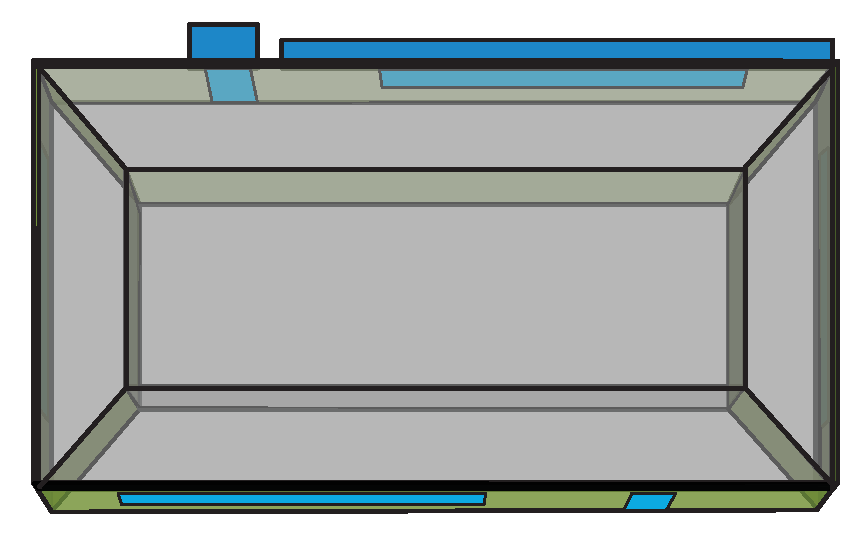
\includegraphics[width=4in]{./Pics/TopView2.eps}
\caption{The office model: top view.}
\label{fig:office1}
\end{figure}

\begin{figure}[h]
\centering
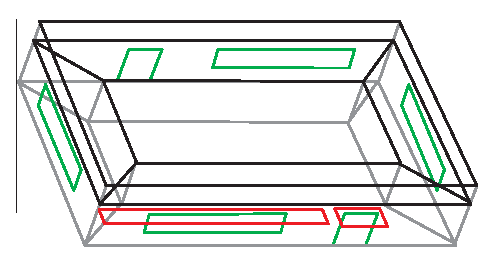
\includegraphics[width=4in]{./Pics/SideView.eps}
\caption{The office model: side view.}
\label{fig:office2}
\end{figure}

\begin{figure}[h]
\centering
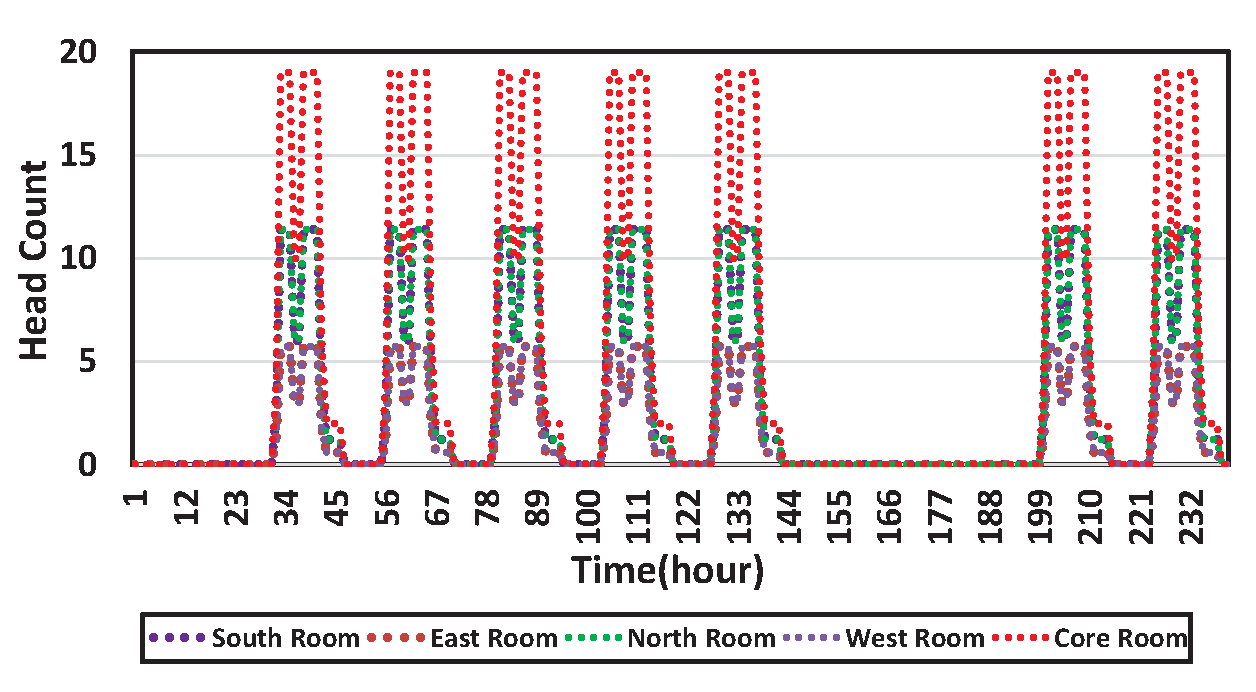
\includegraphics[width=4in]{./Pics/Headcount.eps}
\caption{Occupation information of 5 rooms for 10 days.}
\label{fig:Headcount}
\end{figure}

\begin{figure}[h]
\centering
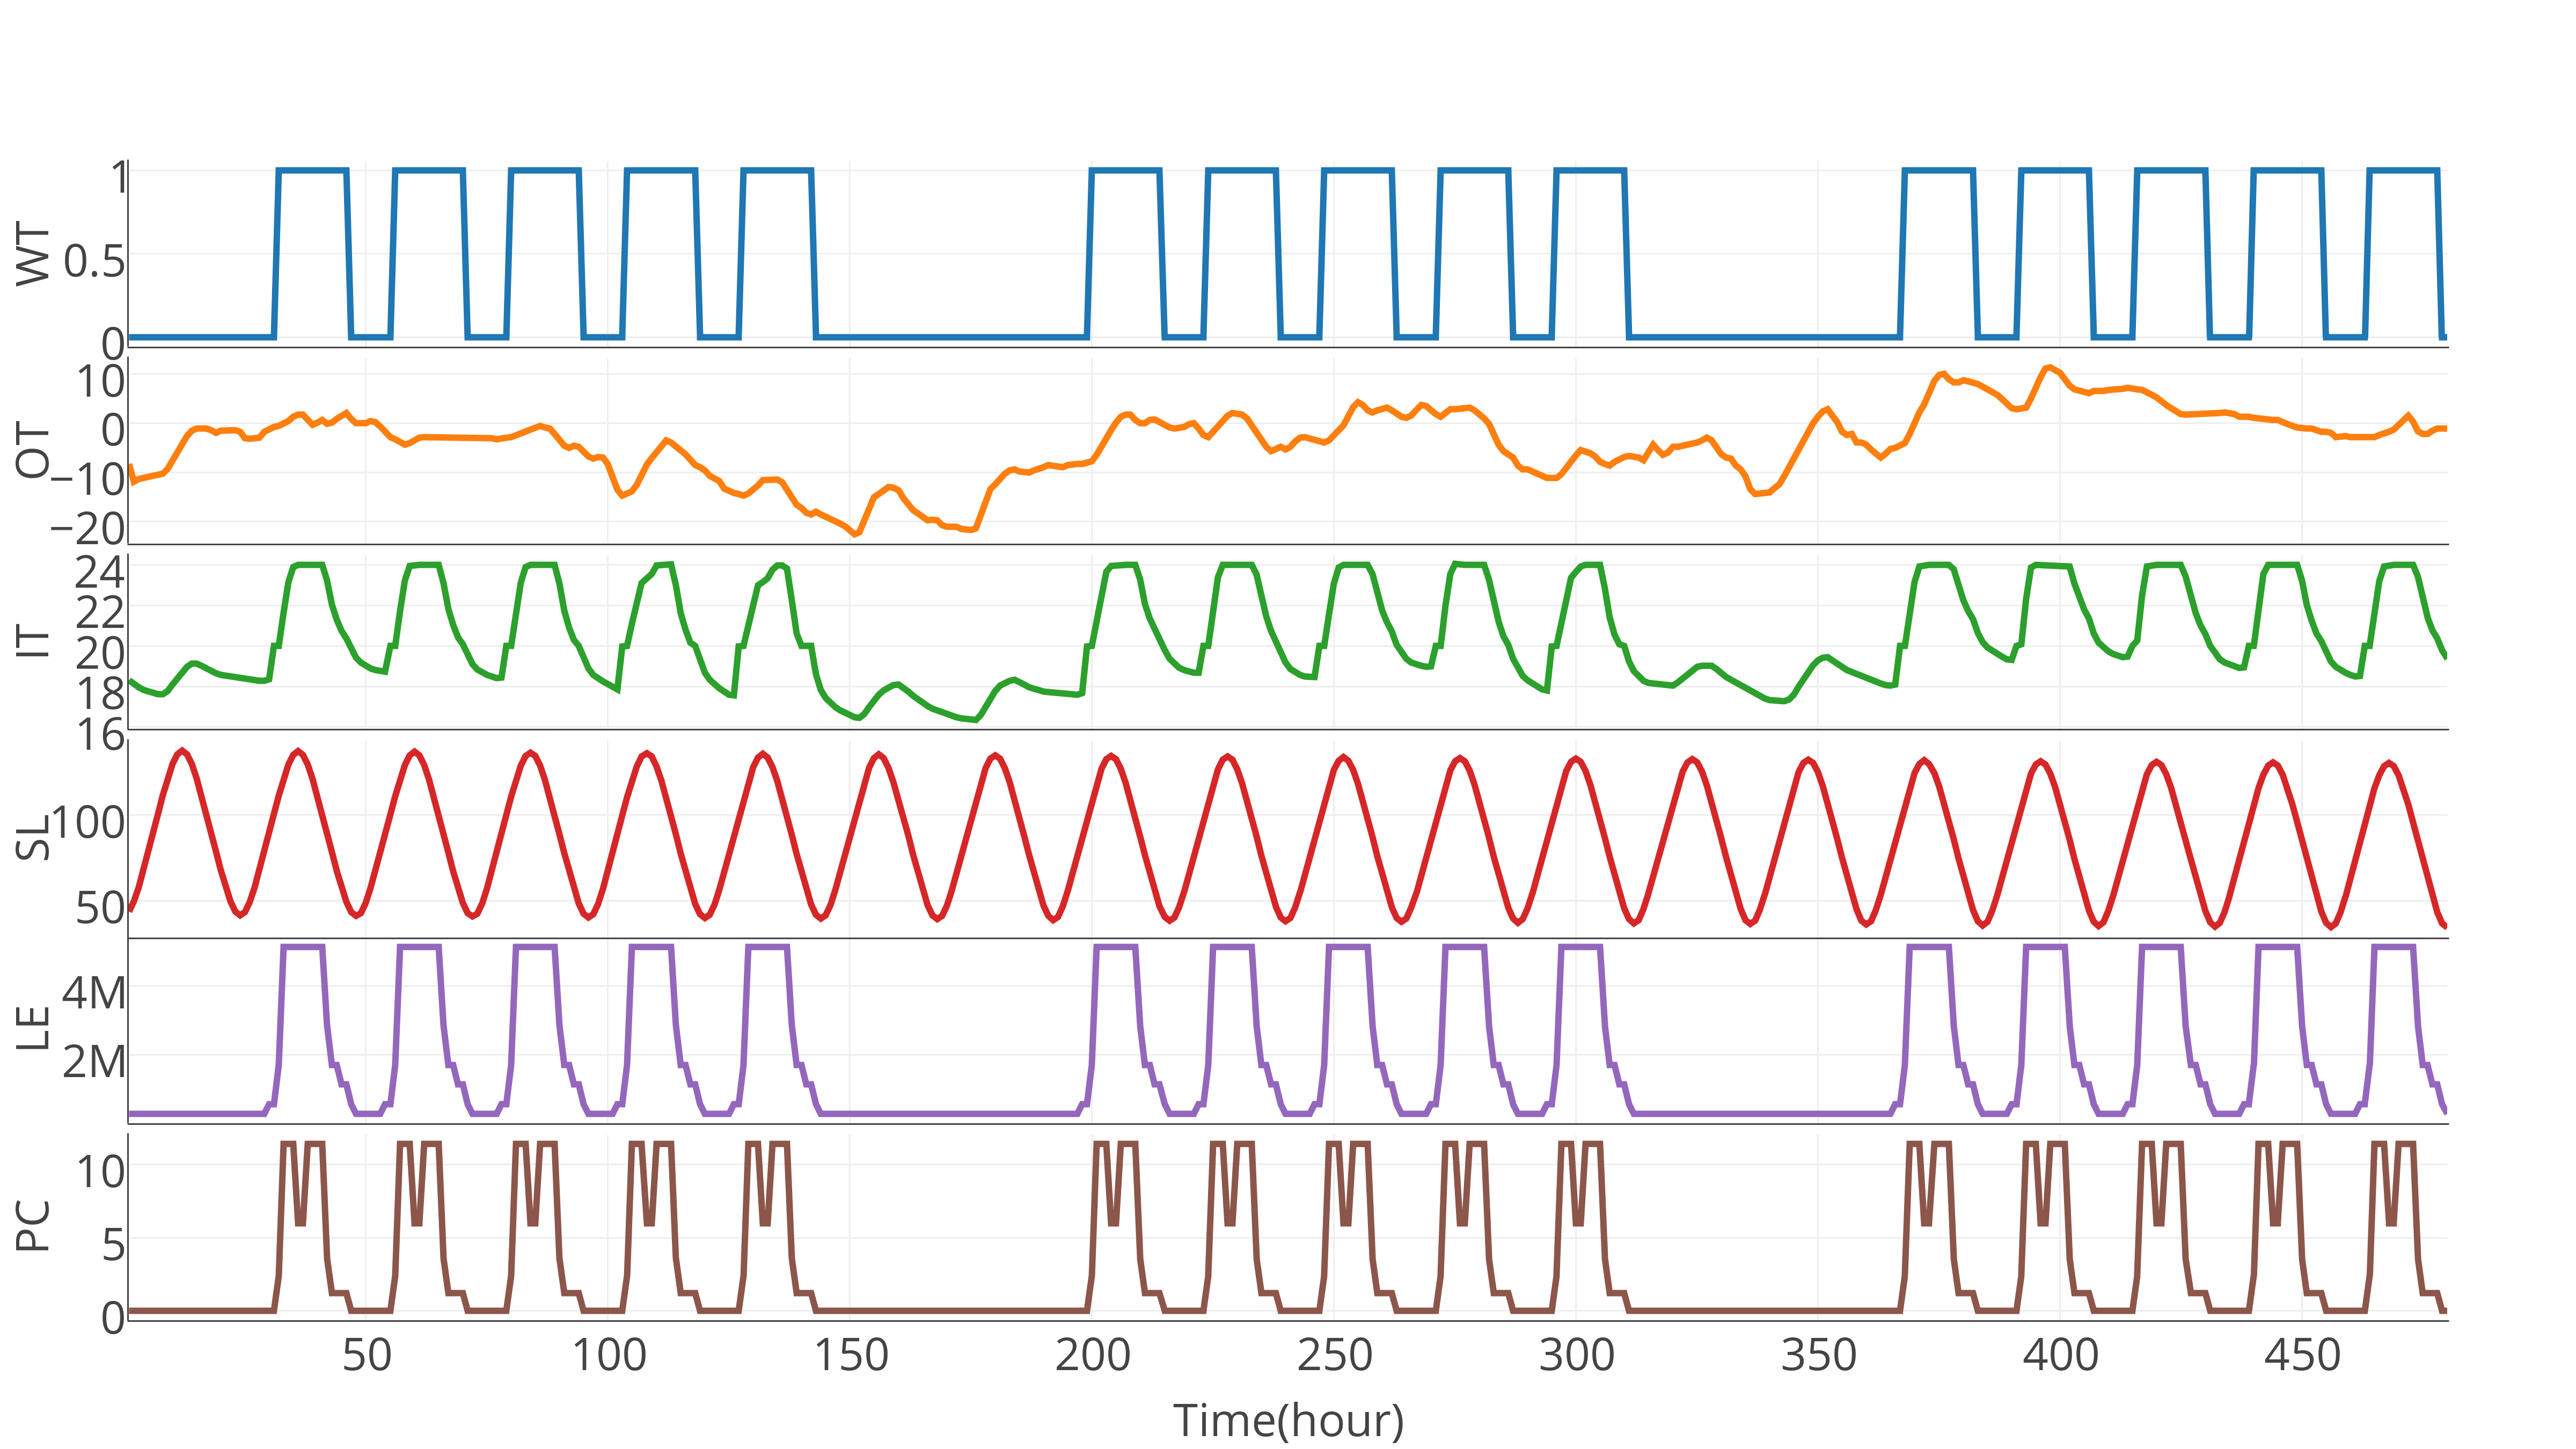
\includegraphics[width=4in]{./Pics/Feature3.eps}
\caption{Selected EnergyPlus input and simulated temperature output data sample in 20 days. (WT: Work Time; OT: Outdoor Temperature; IT: Indoor Temperature; SL: Solar Angle; LE: Lights Energy; PC: People Count.)}
\label{fig:feature}
\end{figure}

In the machine learning model we built for occupancy detection, we carefully selected 5 features each of which possesses some unique information hidden inside. The features are solar angle, indoor temperatures, outdoor temperatures, working time, and lights energy. Solar angle is believed to have periodic information which varies across the entire year, outdoor temperature is an apparent factor that impacts the indoor temperature, working time denotes whether regular working schedule is executed, and lights energy gives out a radiation metric that causes rise of the temperature.

Fig.~\ref{fig:office1} and Fig.~\ref{fig:office2} show the side view and the top view of the building which contains five rooms and HVAC system by using the software EnergyPlus. This building can be influenced by heat sources produced from occupants, electric equipment, air filtration, etc. The weather (ambient temperature and solar effects) affects the room temperature as well. Through the HVAC system with coil and fan, room temperature can be administered properly to ensure that a comfortable temperature in the environment can be produced in the room.

In this room the solar angle ${\theta _s}$ is defined as the angle between the zenith and the centre of the sun disc
\[\cos {\theta _s} = \sin \phi \sin \delta  + \cos \phi \cos \delta \cosh \]
where $h$ is the hour angle in the local solar time, $\delta$ is the current declination of the sum, and $\phi$ is the local latitude. This equation enables us to compute the feature solar angle and all the variables are correlated to the location of the building.

Working time is a feature that determines if the time detected is local working time or not, and it apparently affect the number of working people in a certain office. It is also convenient to achieve schedule of an ordinary worker in an office within the building and it is a good feature contributing to the detection. When a feature is being considered to be incorporated in the feature pool, we first figure out the convenience and difficulty in acquiring the data set. Here working time has a strong correlation with the employee common schedule, which is a relatively data set to acquire. Therefore, working time is chosen as a feature element in the feature pool, and it is even a basic feature owing to its convenience.

Outdoor temperatures are off-the-rack data set collected from weather forecast which also are the inputs for EnergyPlus to generate indoor temperatures data as an output. In this paper, we use the outdoor temperature data set of the location of the building in Chicago, so as our simulated building model goes through the exact same weather conditioning the genuine building has gone through. And outdoor temperatures also plays an instrumental feature role in detection, because it directly influences the indoor temperature, which has a non-linear relationship with the number of employees in a certain office.

The indoor temperature turns out to be one of the key features used in the detection model, to be more accurately, all of the factors including employee occupancy constitute the list of elements that results in the fluctuation of temperature inside the building. In essence, the approach to achieve the detection for a number of employee in a certain room is based on the contribution of heat emitted from different number of employees in a certain room. Owing to the fact that different number of employees gives out different amount of heat to impact the indoor temperature, makes the approach viable to detect the occupancy combing other factors that affect the indoor temperature.

Lights energy is the fifth feature in the feature pool, and it is different from the first four. The first four features are quite convenient features to acquire where the measurement of lights energy is comparatively inconvenient to acquire. However, we want to make the detection more versatile and can be applied in different situations. Despite the inconvenience of data set of lights energy, it is an important metric related to number of employees in a specific office as well. Aiming at provide a more accurate detection, the lights energy feature is incorporated into the feature pool.

As listed above, five features are applied in the machine learning method we apply in our approach. In keeping with different degree to application, different combination of features are used in the methods, which makes the application more flexible.

\subsection{Data Configuration}
\begin{figure}[!h]
\centering
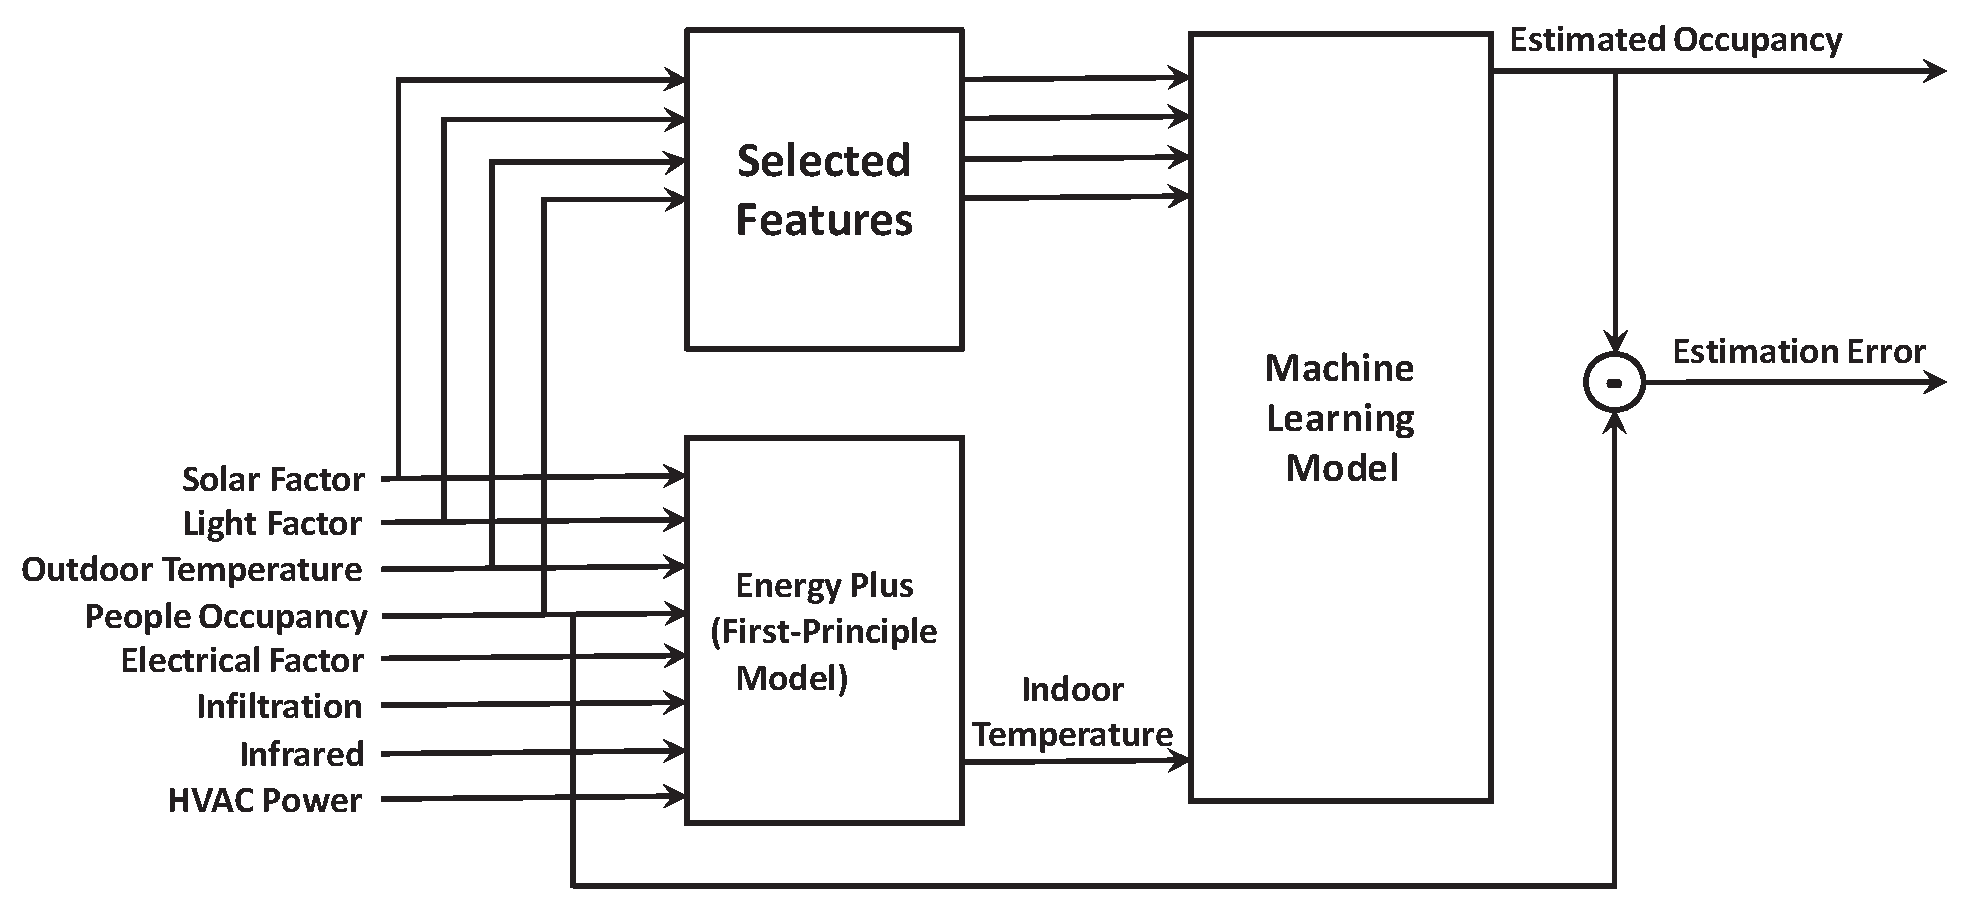
\includegraphics[width=4in]{./Pics/FlowDiagram2.eps}
\caption{Data configuration of machine learning model.}
\label{fig:SVRFlow}
\end{figure}

Fig.\ref{fig:SVRFlow} shows how EnergyPlus produces indoor temperature in a certain room specifically. EnergyPlus feeds off factors such as indoor temperature, solar factor, electrical factor, light factor, infiltration, infrared, and people occupancy before it produces indoor temperature as an output using built-in methods and methods in accordance with its inputs. Of all those features taken into the method, indoor temperature is the key feature because it is directly impacted by the increase or drop in the number of employees in a certain office.

In general, the machine learning model takes the selected parameters as its features to train the data and yield results. It is highlighted that the relationship between occupancy and other factors are non-linear related, where SVR and neural network are a good choices to solve a non-linear problem used for detection. And machine methods are increasingly used in all kinds of supervised and unsupervised problems in all aspects.

Fig.~\ref{fig:Headcount} shows a vintage working schedule of the five zones of an office building. Our goal of the detection model is to detect accurate number of employees in a room by certain parameters and data collections. Fig.~\ref{fig:feature} shows the simulated temperature curves and input curves over 20 days from EnergyPlus for a smart building model with the five separate zones shown in Fig.~\ref{fig:office2}. The schedule for each room can be assigned differently by EnergyPlus. The selected features are then combined together to occupancy behavior in the smart building. In general, the SVR model takes the selected features as its parameters to train the data and yield the corresponding results. It should be noted that there is a nonlinear relationship between the occupancy and the related factors. The machine learning model can be used to solve this nonlinear problem used for occupancy detection.

In this model, we provide two sets of model which offers different extent of convenience to detect number of employees in an office. The first set of model is comprised of features such as solar factor, working time, indoor temperature and outdoor temperature, data of which can be acquired through sole mathematic computation and EnergyPlus simulation. It is relatively convenient to obtain all the features required in the first feature set. However, we introduce one more features in the second feature set, light factor, to enhance the accuracy of model. Light factor requires the model to learn overall energy that light consumes during a certain quantity of time which is a comparatively inconvenient feature to obtain, however, it is capable of making the detection more accurate. It is also highlighted here that all of the data we feed in the model is generated from EnergyPlus or obtained through mathematical calculation, thus further experiments are likely to be conducted in real-life data condition.

For separating the whole data set, we split the one-year simulation data into twelve months and three time periods, in which the months 1-3, 5-7, 9-11 are referred to as the training data and the months 4, 8, 12 are specified for the testing data in the proposed machine learning model.

\section{Support Vector Regression Results and Analysis}
In this section, we will illustrate how we measure error variation for the proposed SVR model and discuss the effectiveness of applying different number of features in this model.

\subsection{Experiment Results}
\begin{table}[!h]
\label{table:training}
\caption{Training error statistics of SVR model using different numbers of feature}
\centering
\begin{tabular}{m{1.2cm}m{0.8cm}m{0.8cm}m{0.8cm}m{0.8cm}m{0.8cm}m{0.8cm}}
\hline
& \multicolumn{2}{c}{$C$=100} & \multicolumn{2}{c}{$C$=500} & \multicolumn{2}{c}{$C$=1000} \\
\cline{2-7}
Features &   \hspace{0.2cm} 4  &\hspace{0.2cm}   5  &\hspace{0.2cm}   4  &\hspace{0.2cm}   5  &\hspace{0.2cm}   4  & \hspace{0.2cm}  5  \\
\hline
Avg. error&0.721& 0.310   & 0.576 &  0.326   &  0.550  &  0.348        \\
Err. ratio&0.311& 0.0856  & 0.188 &  0.0889  &  0.181  &  0.124        \\
\hline
\end{tabular}
\end{table}


\begin{table}[!h]
\label{table:testing}
\caption{Validation error statistics of SVR model using different numbers of feature}
\centering
\begin{tabular}{m{1.2cm}m{0.8cm}m{0.8cm}m{0.8cm}m{0.8cm}m{0.8cm}m{0.8cm}}
\hline
& \multicolumn{2}{c}{$C$=100} & \multicolumn{2}{c}{$C$=500} & \multicolumn{2}{c}{$C$=1000} \\
\cline{2-7}
Features &   \hspace{0.2cm} 4  &\hspace{0.2cm}   5  &\hspace{0.2cm}   4  &\hspace{0.2cm}   5  &\hspace{0.2cm}   4  & \hspace{0.2cm}  5  \\
\hline
Avg. error&0.819& 0.317   & 0.694 &  0.330   &  0.638  &  0.390        \\
Err. ratio&0.068& 0.0264  & 0.0578 &  0.0274  &  0.0532  &  0.0325        \\
\hline
\end{tabular}
\end{table}

In this part of section, we evaluate the SVR detection model using testing data set. Through a wide range of experiments, we learn radial basis function kernel also known as Gaussian kernel work best in this model. The most important two parameters in SVR model is penalty $C$ and radius $\varepsilon$ where plenty of tests are conducted to obtain a good set of parameter, hence, we experiment different values of $C$ and $\varepsilon$ hoping to obtain the best. It is widely known that to get an accurate performance in SVR model or any other machine learning methods, the best approach is to enumerate a quantity of combinations of parameters, and conduct experiments to drive the result toward a better trend. During the process of seeking out the best result for the model, the set of parameters is adjusted step by step to obtain a model which has a better accuracy than the previous one. After a batch of experiments for the model are conducted, we pick out the parameters in the model that brings about the best performance. Here we also want to highlight, that most of the time, the parameters working best for a model sometimes can not be proved theoretically, therefore confirmed parameters often are determined by a great number of trials and experiments.

Table \rom{1} shows the training error statistics of the proposed SVR model used for occupancy detection. Some comparisons between two sets of features are apparently displayed from the results shown in this table. Numerical simulation shows that $\varepsilon$ being equivalent to 0.01 is a reliable choice for this SVR-based occupancy model. At each sample point, the estimation error ${e_i}$ is defined as ${e_i} = \left| {O_i^{SVR} - O_i^{EP}} \right|$ where $O_i^{SVR}$ denotes the occupancy value obtained by the proposed SVR model and $O_i^{EP}$ denotes the real value of occupancy generated from EnergyPlus.
We calculate the average error and the error ratio by $\frac{1}{n}\sum\nolimits_n {{e_i}}$ and $\frac{{Average{\kern 1pt} {\kern 1pt} {\kern 1pt} {\kern 1pt} error}}{{full{\kern 1pt} {\kern 1pt} {\kern 1pt} {\kern 1pt} occupancy}}$, respectively. Also, in this table different values of $C$ are tested to seek out an accurate model for occupancy detection.

Table \rom{2} shows the validation error statistics of the proposed SVR model. The reason why the 5-feature model performs even better than the 4-feature model for occupancy detection is that the 4-feature model suffers slightly in under-fitting issue which results in a high bias. It is important to determine the parameters which can maintain a balance between under-fitting and over-fitting.
\subsection{Analysis}
\begin{figure}[h]
\begin{minipage}{\textwidth}
\centering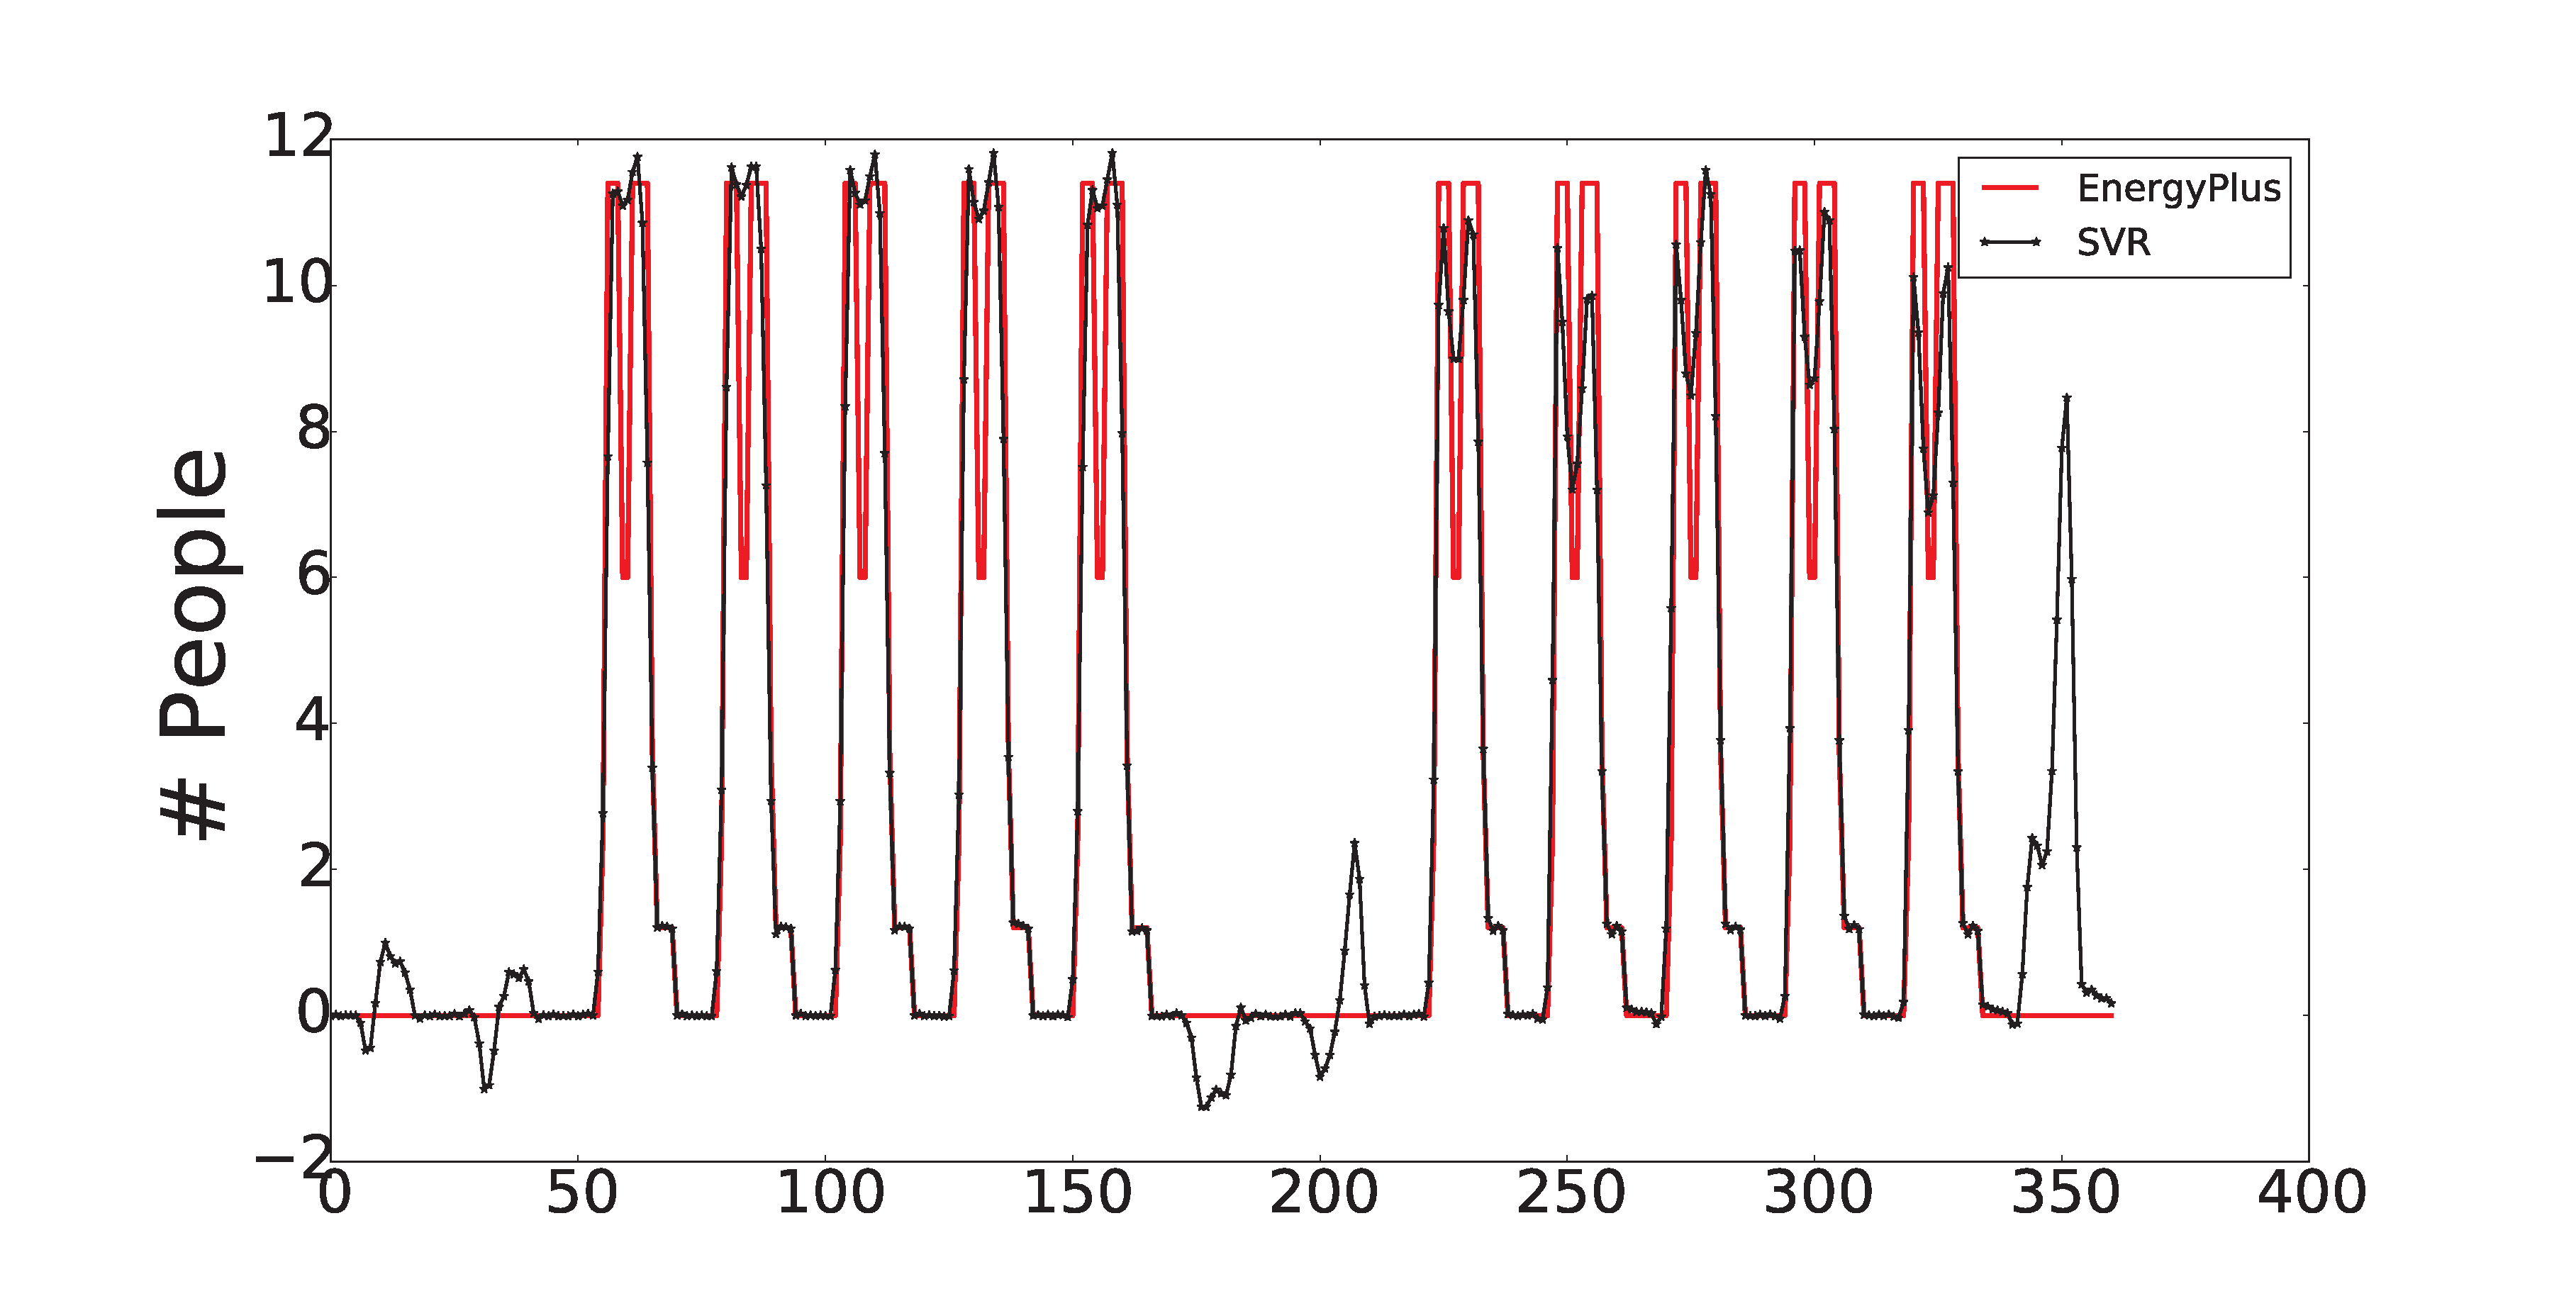
\includegraphics[width=5in]{./Pics/100C4Features.eps}
\subcaption{}\label{fig:1a}
(a) 4 features.
\end{minipage}
\hfill

\vspace{3ex}

\noindent\begin{minipage}{\textwidth}
\centering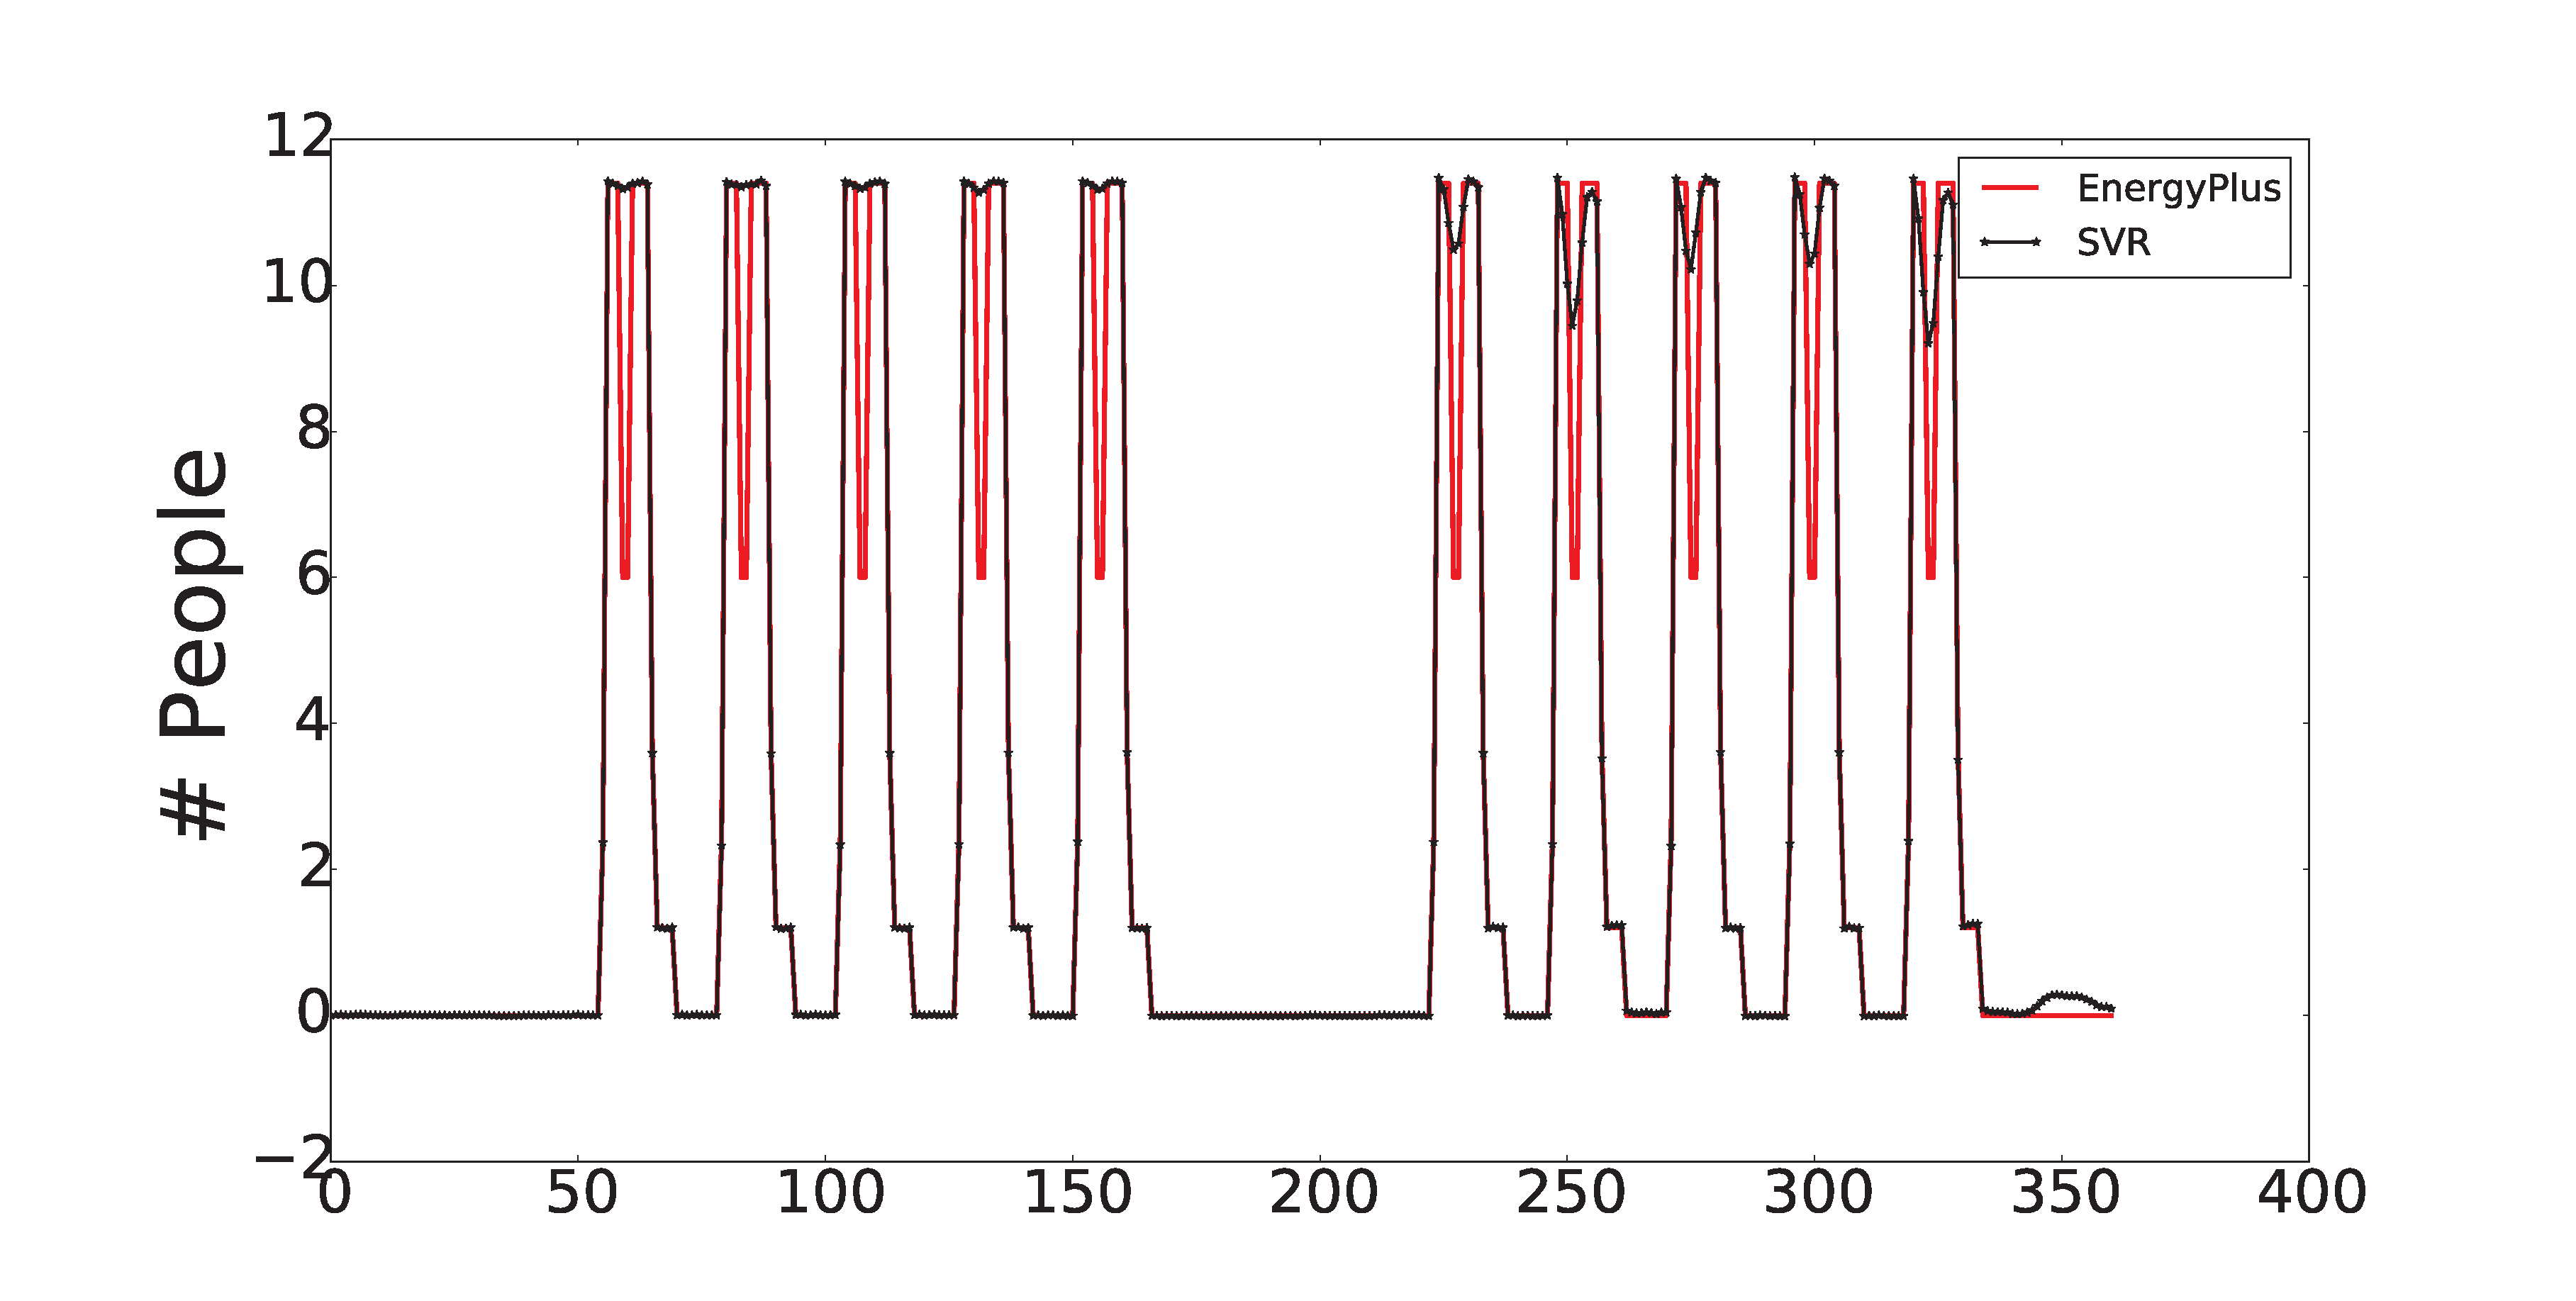
\includegraphics[width=5in]{./Pics/100C5Features.eps}
\subcaption{}\label{fig:1b}
(b) 5 features.
\end{minipage}
\hfill
\caption{Occupancy estimation accuracy when $C$ equals 100 using SVR with 4 features and 5 features.}\label{fig:compare1}
\end{figure}

\begin{figure}[h]
\begin{minipage}{\textwidth}
\centering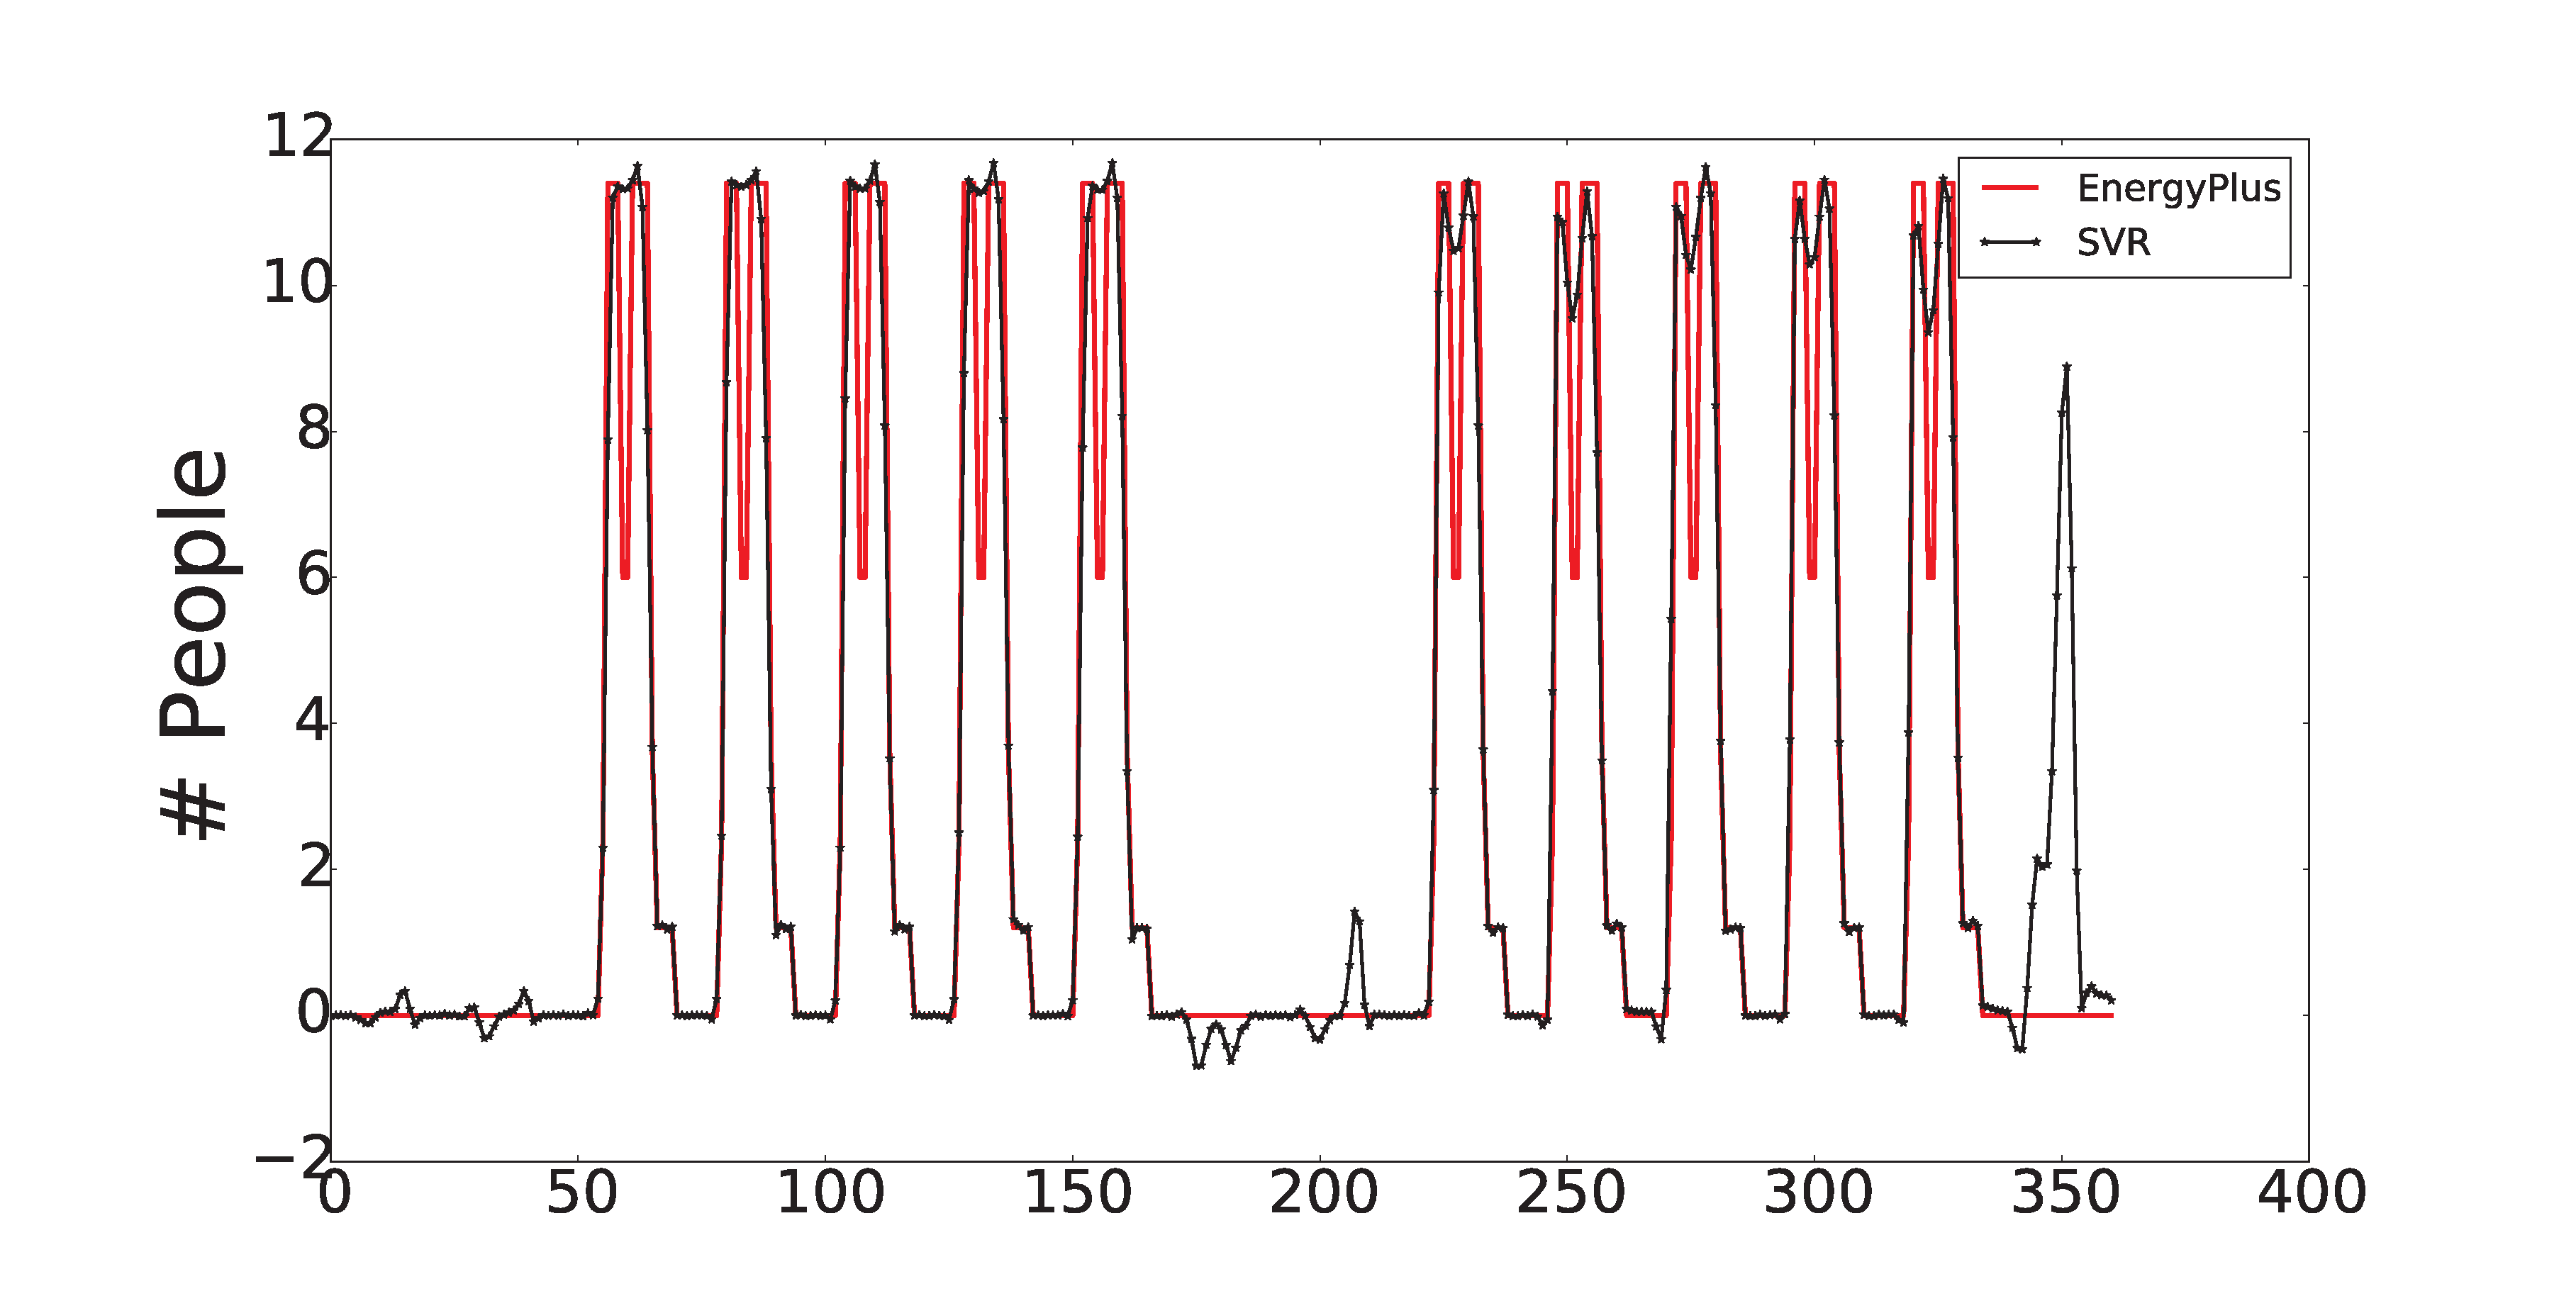
\includegraphics[width=5in]{./Pics/500C4Features.eps}
\subcaption{}\label{fig:1a}
(a) 4 features.
\end{minipage}
\hfill

\vspace{3ex}

\noindent\begin{minipage}{\textwidth}
\centering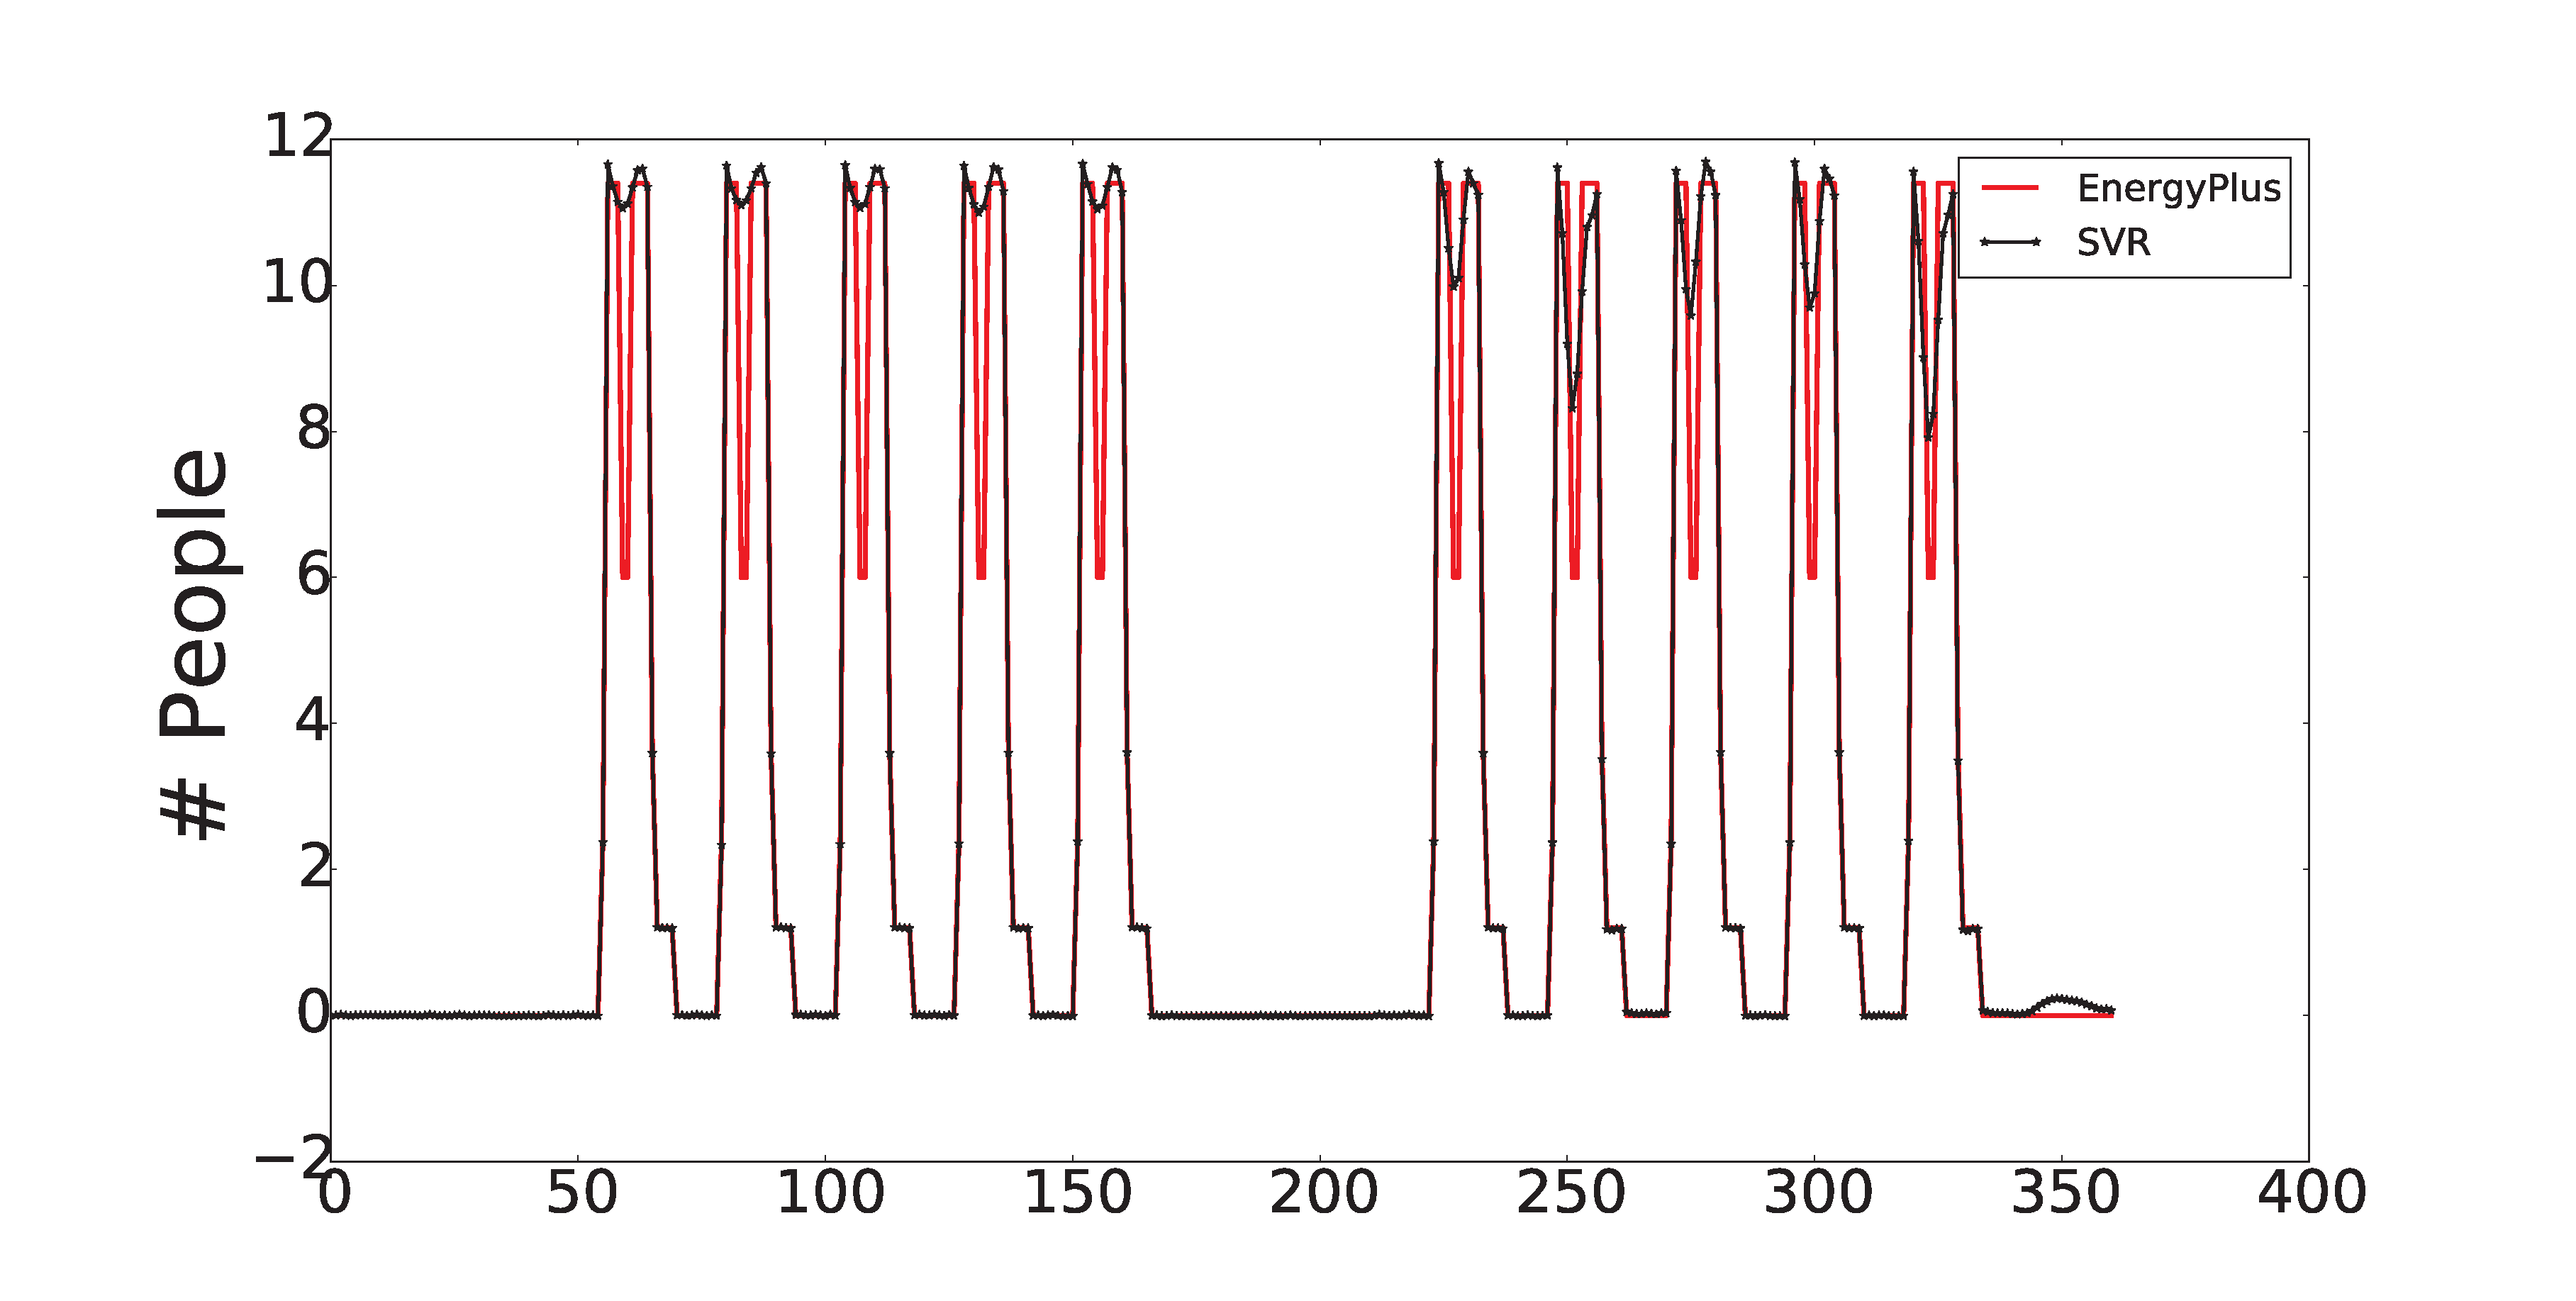
\includegraphics[width=5in]{./Pics/500C5Features.eps}
\subcaption{}\label{fig:1b}
(b) 5 features.
\end{minipage}
\hfill
\caption{Occupancy estimation accuracy when $C$ equals 500 using SVR with 4 features and 5 features.}\label{fig:compare2}
\end{figure}

\begin{figure}[h]
\begin{minipage}{\textwidth}
\centering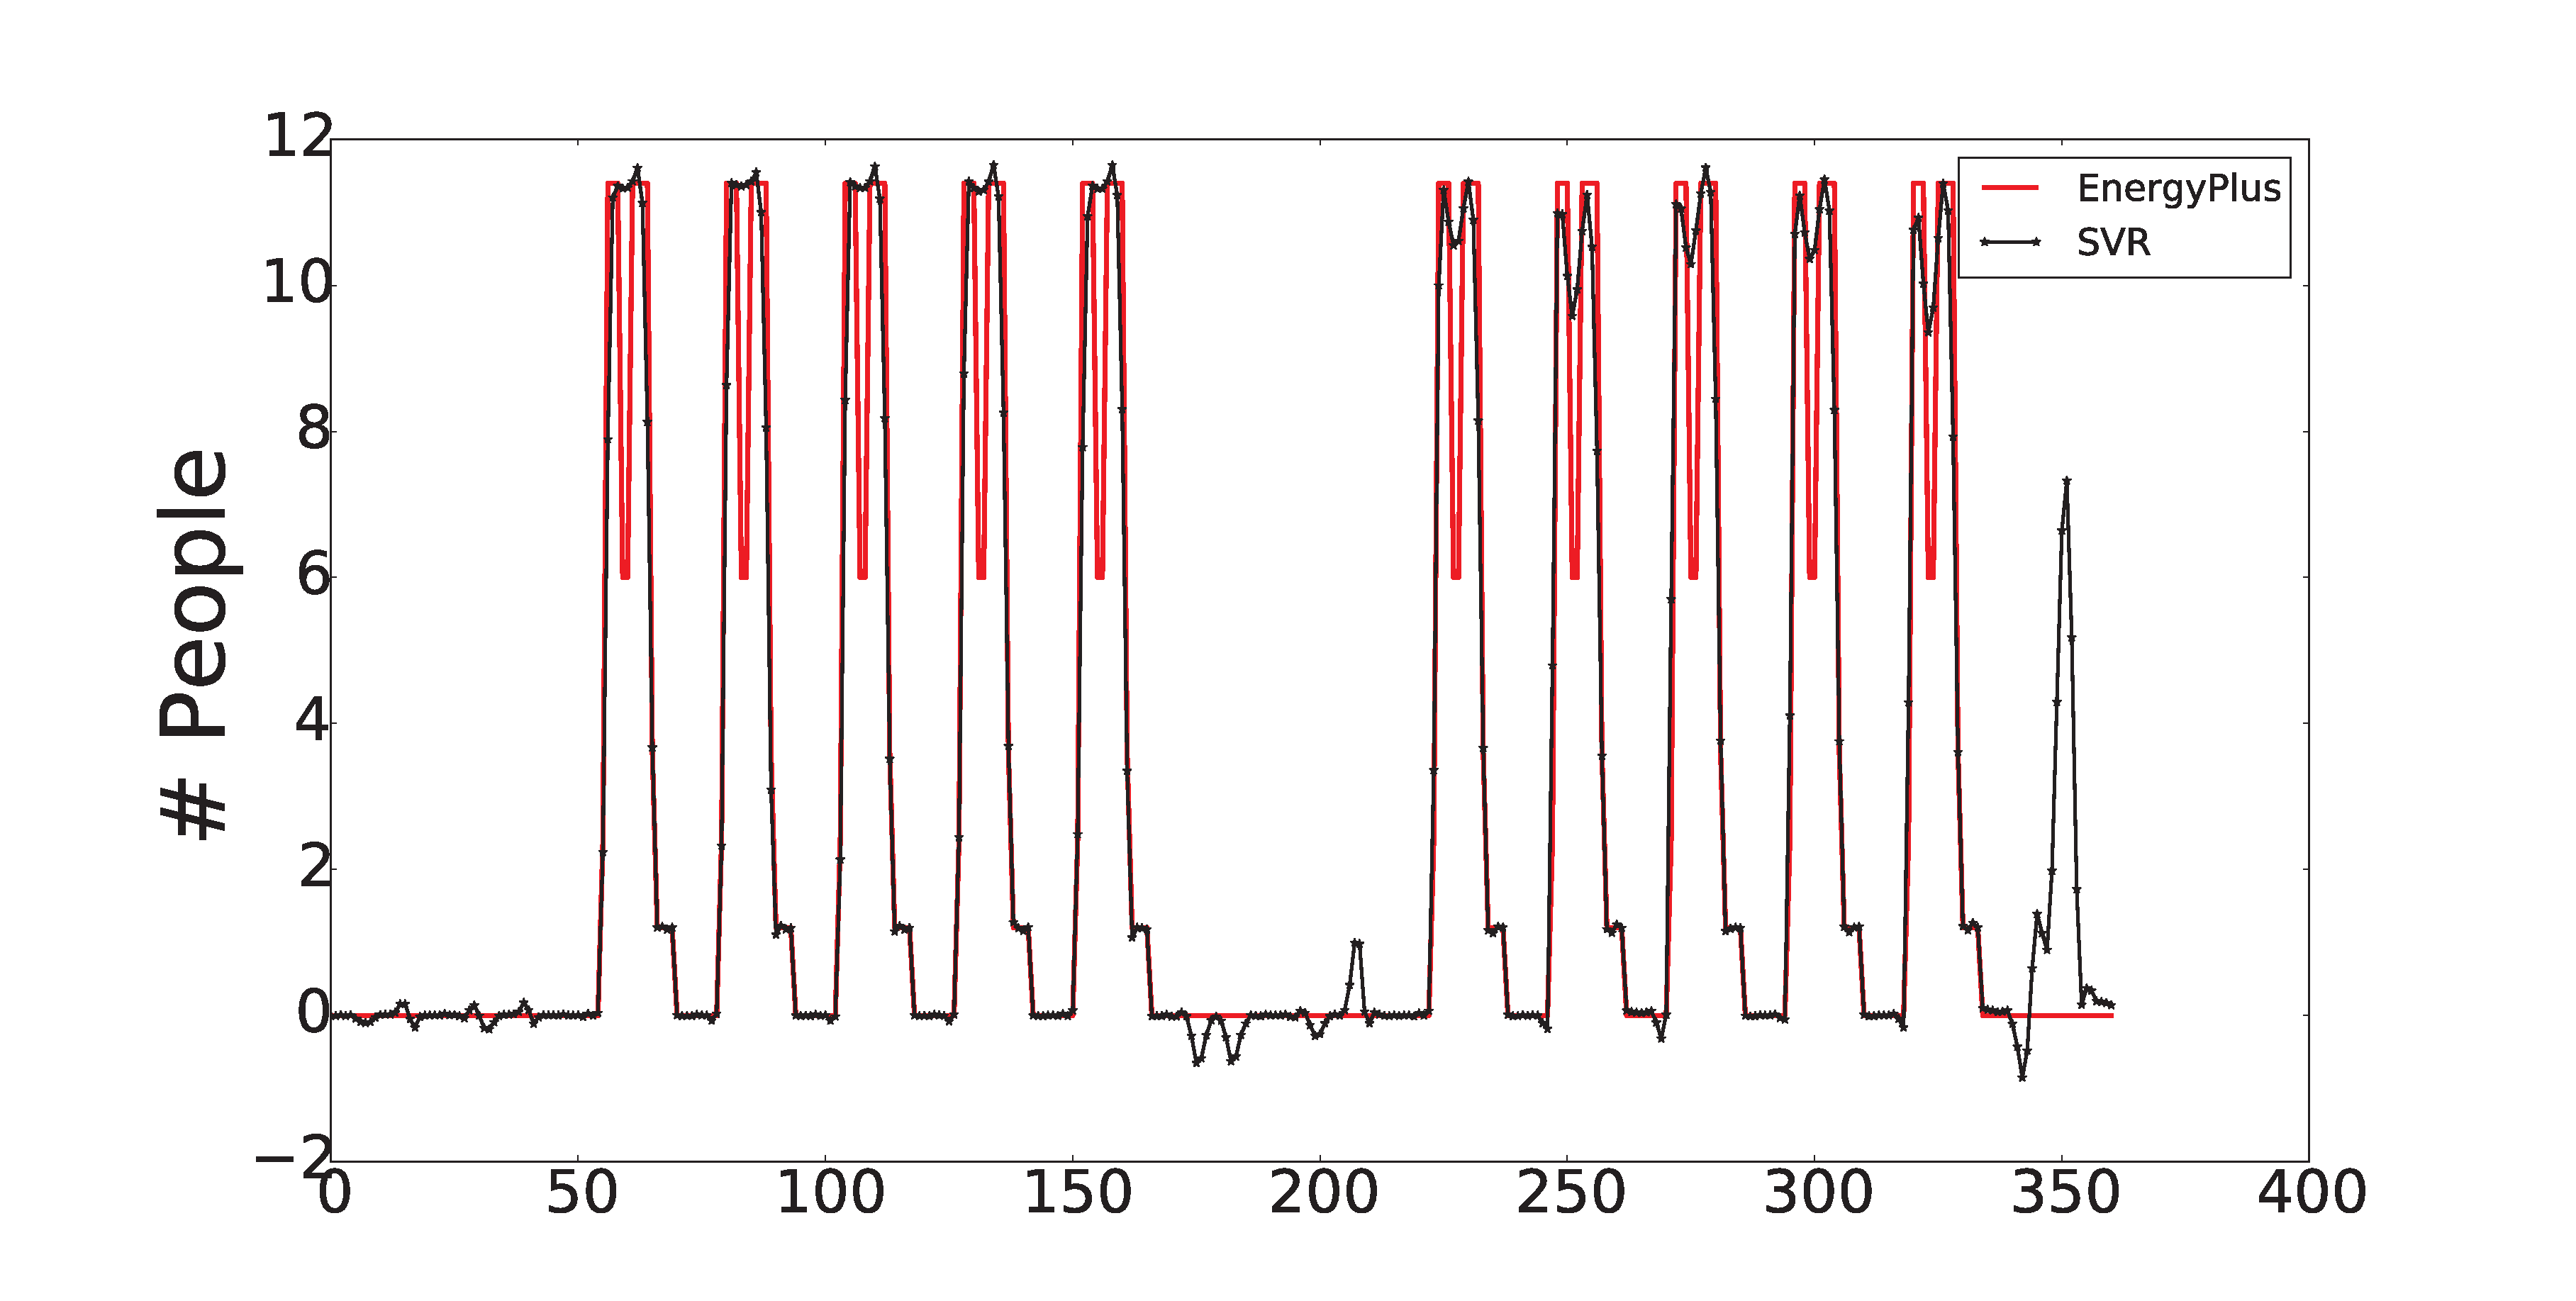
\includegraphics[width=5in]{./Pics/1000C4Features.eps}
\subcaption{}\label{fig:1a}
(a) 4 features.
\end{minipage}
\hfill

\vspace{3ex}

\noindent\begin{minipage}{\textwidth}
\centering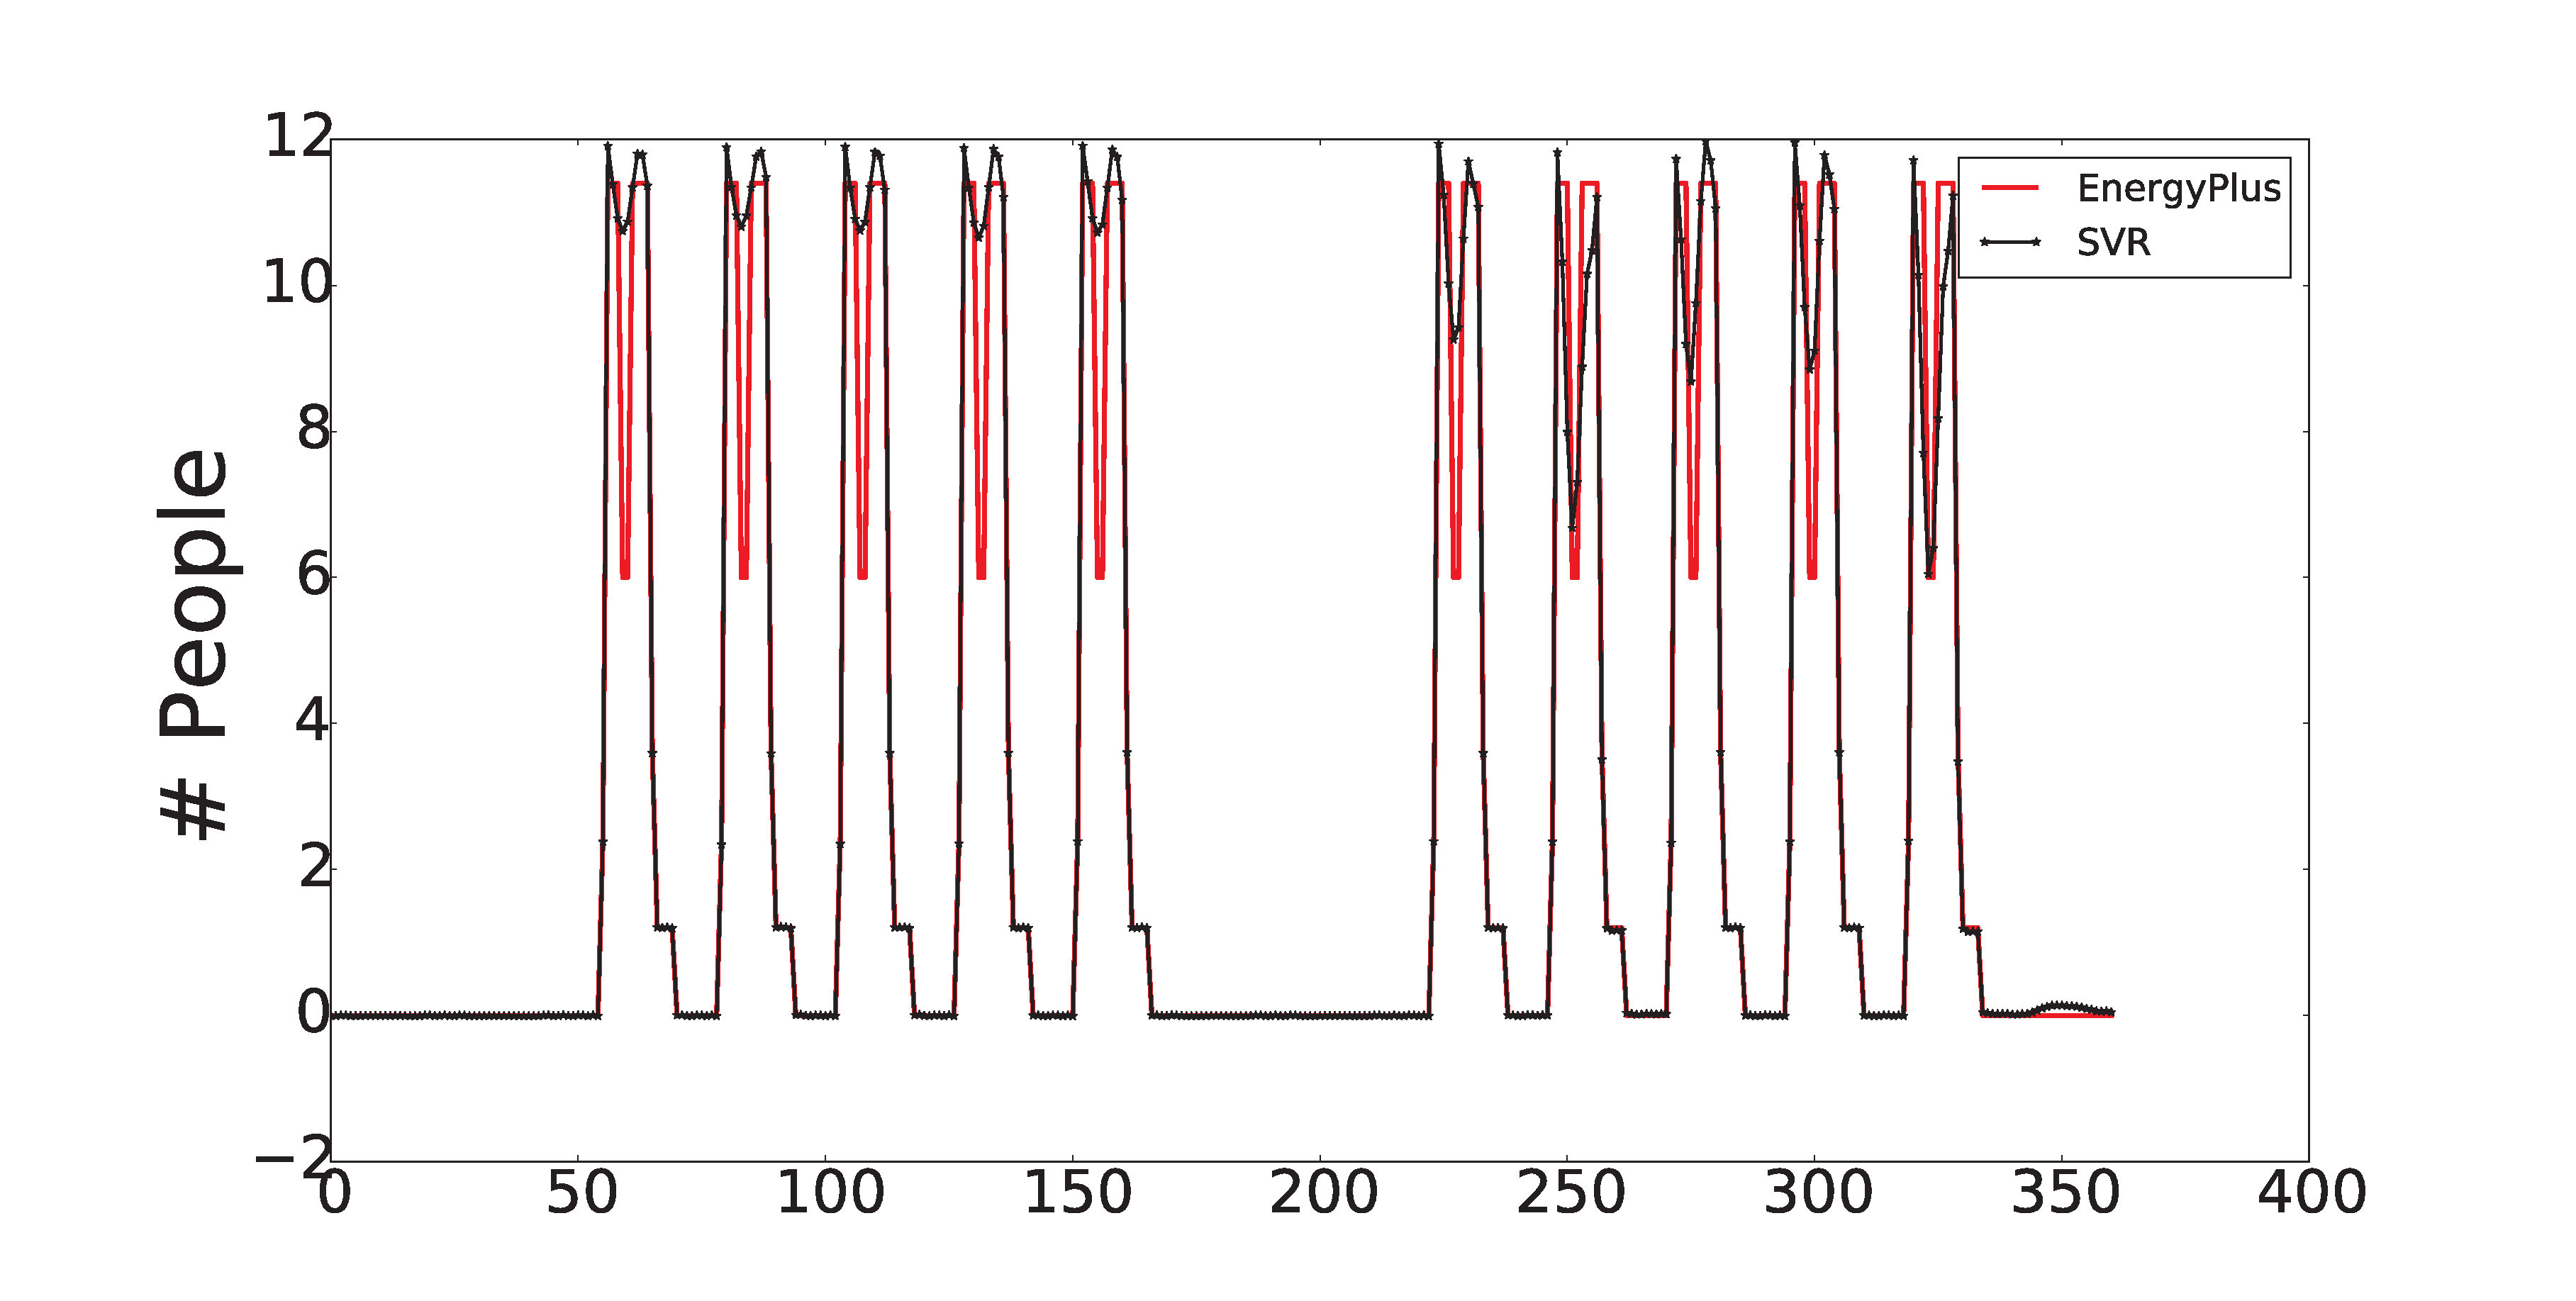
\includegraphics[width=5in]{./Pics/1000C5Features.eps}
\subcaption{}\label{fig:1b}
(b) 5 features.
\end{minipage}
\hfill
\caption{Occupancy estimation accuracy when $C$ equals 1000 using SVR with 4 features and 5 features.}\label{fig:compare3}
\end{figure}
In the second part of the section, the process of achieving the best model we build is revealed, and several figures of performance for models is displayed to have a direct comparison for the model under different number of figures. The figures mainly display the accuracy of applying 4 features or 5 features in the model, and offers a vivid comparison in those figures.

We now display the accuracy of applying 4 features or 5 features in the proposed SVR model. To obtain the best parameter setting in the SVR model used for occupancy detection, we need to constantly compare the gap between the training and testing errors for the collected data sets by EnowergyPlus. If the gap of accuracy between training and testing errors are relatively large, which means that this model is over-fitting on the training data. In accuracy on training data implies that the model has a potential under-fitting. In this situation, we need to adjust parameters to make the SVR-based model work better.

We randomly pick out a 15-day period from the testing data set and compare it to the genuine value generated by EnergyPlus. Large number of experiments in this proposed SVR model shows that 0.01 is a stable-performing value for $\varepsilon$. Fig. \ref{fig:compare1}, Fig. \ref{fig:compare2}, and Fig. \ref{fig:compare3} show the simulation results of occupancy detection accuracy of SVR model by using different numbers of feature. To find a better performance model, we set $C$ to be 100, 500, and 1000, respectively. Simulation results show that the SVR model tends to become more complex when the value of $C$ becomes larger, hence the goal of optimizing the SVR model is to find the value of $C$ that is one better tradeoff between under-fitting and over-fitting. For the 5-feature model, it can be seen that the SVR model can obtain better performance for occupancy detection when the value of $C$ varies in the range from 10 to 1000.

The two sets of features provide different convenience in detecting to meet different demand. The first set of features are features can be relatively easily acquired while the second requests more efforts. The first set of feature only requires data set that can be obtained from mathematic computation, whereas the second set of features requires light energy which is a set of statistics that needs more effort to achieve. In terms of practical application, it is suggested to choose the one that meets demand and gives the best convenience. However, further improvement can be considered by building model revolving around absorbing the current data set into the SVR model, which makes the model work as a dynamic equation that is able to self-improved by newly absorbed data set and remain more effectively according to the current circumstance. Most importantly, it is suggested to choose the most efficient approach based on the facing situation, after all, the model is able to fulfill ordinary demand in accuracy in 4-feature model. Further improvement is likely to happen if consider specific conditions for other office in detail.

\section{Neural Network Results and Analysis}
In this section, results of neural network are achieved and explained similarly as it is manifested in last section. The way we measure errors and show the performance of neural network model is a little different owing to the different characteristics of neural network. Further demonstration will expanded in this section, and a set of figures will be shown to judge the performance of neural network.

\subsection{Results}
\begin{figure}[h]
\centering
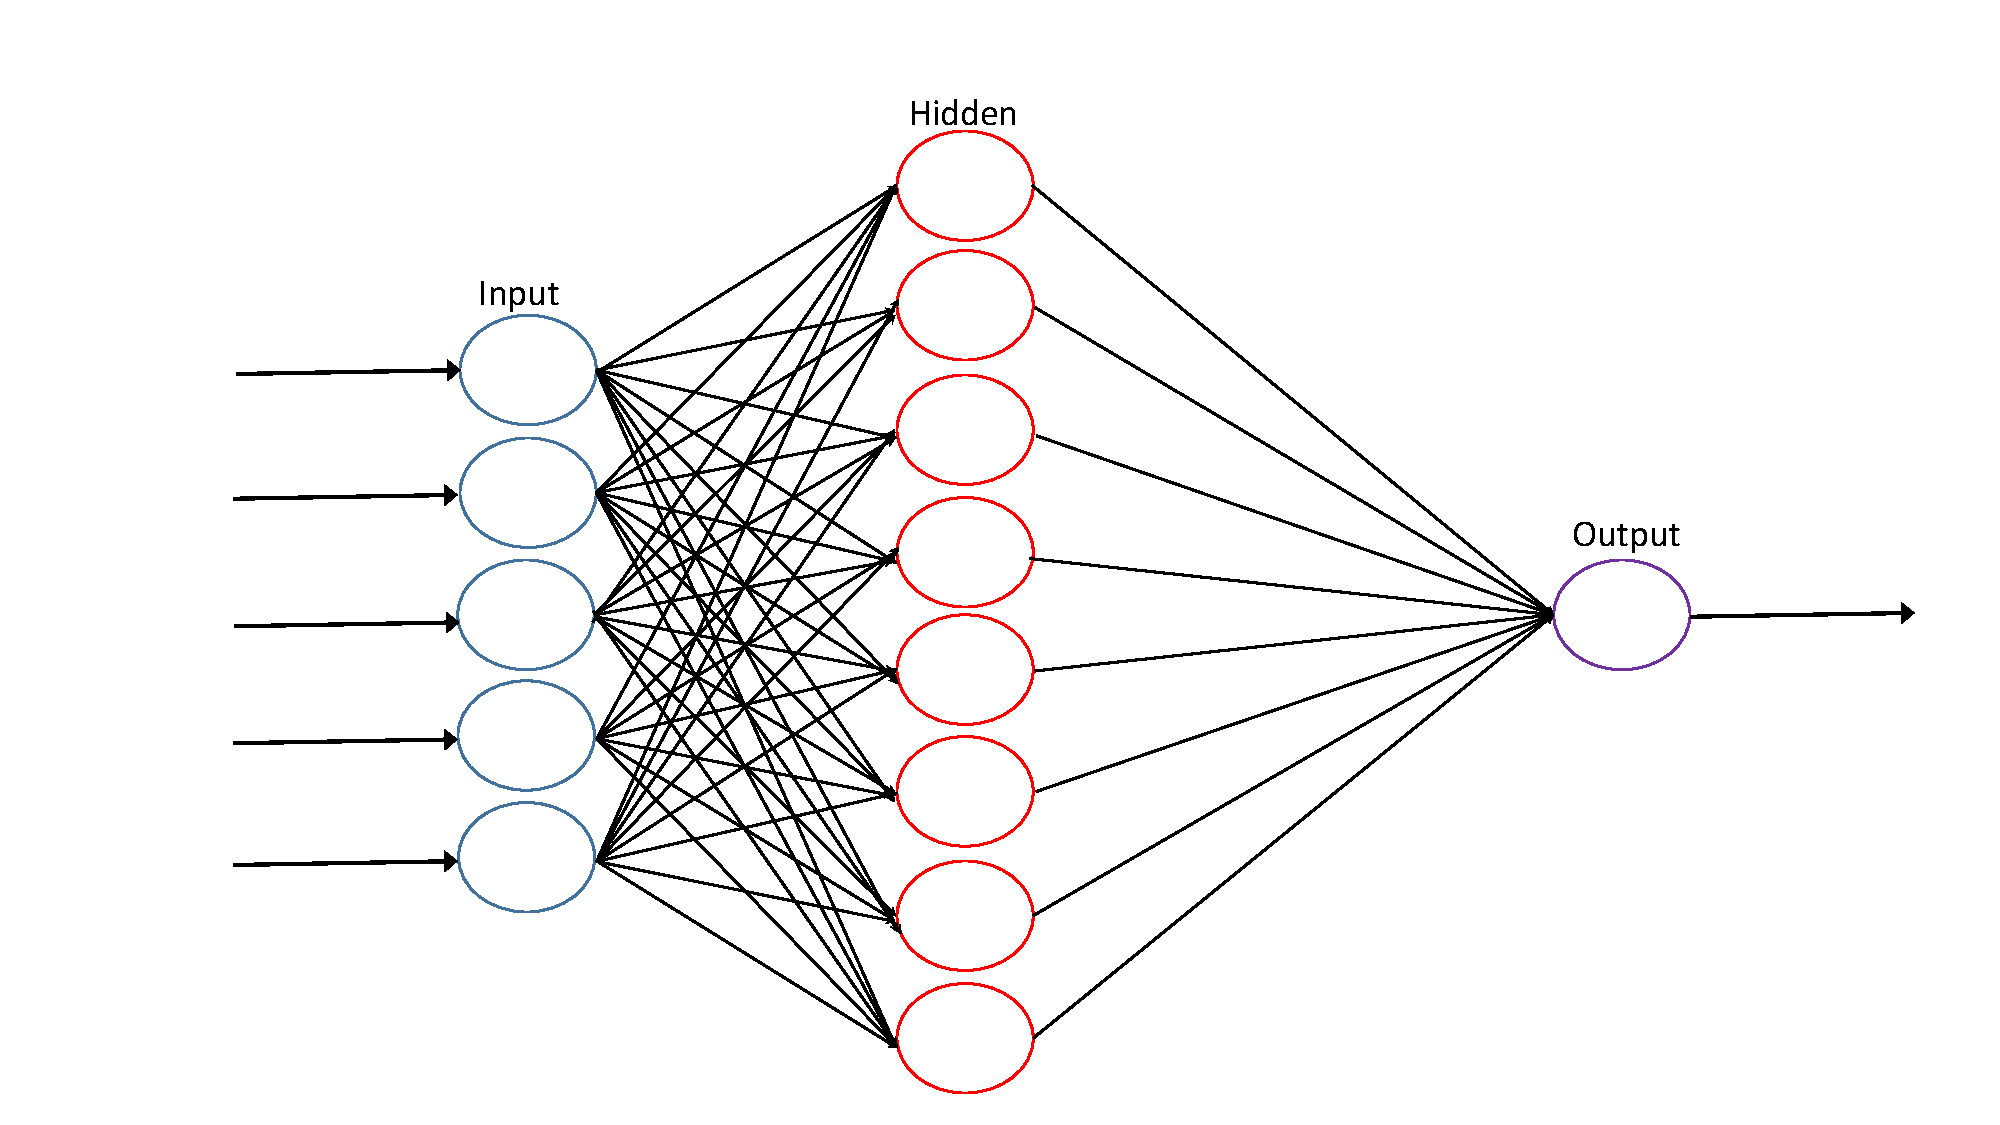
\includegraphics[width=4in]{./Pics/nn.eps}
\caption{Neural Network structure.}
\label{fig:nn}
\end{figure}

In this paper, we use a two-layer feedforward neural network to build up a model which is able to detect the occupancy in a smart building. Fig. \ref{fig:nn} shows the neural network we established possesses 8 sigmoid hidden neurons and linear output neurons. The number of neurons in a hidden layer determines the complexity of a neural network, where the more hidden neurons the more likely that the neural network is to get overfitted. Therefore, in the process of achieving best suitable weights and biases for the model, it is indispensable to apply the early stopping method to obtain a proper set of value for weight and bias. Therefore, the neural network is trained with Levenberg-Marquardt back propagation, which is an method widely used in solving non-linear least squares problems. It is relatively faster to acquire the weights and biases we want to set for the whole model.

The Levenberg-Marquardt approach is a standard method applied to solve nonlinear least squares problems. To minimize the sum of the squares of all errors between detected value and data points, least square problems appear when a parameterized function is required to fit a set of original data points. And nonlinear least squares approaches require an iterative process to improve parameters in a model so as to diminish the sum of the squares of the errors shown between the original data points and function. In essence, the Levenberg-Marquardt curve-fitting approach is virtually a combined technique of two minimiazation methods, the gradient descent and the Gauss-Newton method. The sum of the squared errors is minimized by updating the parameters in the steepest descent direction in gradient descent method. In the Gauss-Newton method, it assumes the least square function as locally quadratic to diminish the sum of the squared errors, thus attempting to seek out the minimum of the quadratic. For the parameters, the Levenberg-Marquardt method uses more like the gradient descent method when there is a large gap between the optimal value and current value, and more like the Gauss-Newton method when there is a small variation between the optimal value and current value.

The method combines advantages of the steepest descent method (that is, minimization along the direction of the gradient) with the Newton method (that is, using a quadratic model to speed up the process of finding the minimum of a function). This method obtained its operating stability from the steepest descent method, and adopted its accelerated convergence in the minimum vicinity from the Newton method. Standard implementation of the Levenberg-Marquardt method (LMA), its drawbacks are discussed below. When minimizing a nonlinear least-squares function, the Levenberg-Marquardt method can suffer from a slow convergence, particularly when it must navigate a narrow canyon en route to a best fit. On the other hand, when the least-squares function is very flat, the method may easily become lost in parameter space. Several improvements to the Levenberg-Marquardt method are used in order to improve both its convergence speed and robustness to initial parameter guesses. We include a geodesic acceleration correction term, explore a systematic way of accepting uphill steps that may increase the residual sum of squares due to Umrigar and Nightingale, and employ the Broyden method to update the Jacobian matrix. We test these changes by comparing their performance on a number of test problems with standard implementations of the method. We suggest that these two particular challenges, slow convergence and robustness to initial guesses, are complimentary problems. Schemes that improve convergence speed often make the method less robust to the initial guess, and vice versa.

The Levenberg-Marquardt method works as an iterative procedure in solving numeric minimization methods. Before starting minimizing an equation, it is required to assign parameter vector $\beta$ an initial value. The initial value assigned for $\beta$ is important because the method is able to converge to a global minimum, under the condition that the initial guess is relatively close to the final solution.

In each iteration step, the parameter vector $\beta$ is substituted by a new estimate, $\beta + \delta$. To find $\delta$, the functions $f\left( {{x_i},\beta  + \delta } \right)$ are approached by their linearizations
\[f\left( {{x_i},\beta  + \delta } \right) \approx f\left( {{x_i},\beta } \right) + {J_i}\delta \]
where
\[{J_i} = \frac{{\partial f\left( {{x_i},\beta } \right)}}{{\partial \beta }}\]
works as the gradient of $f$ with respect to ��.

Working through some mathematical computations and reductions, we can get equation
\[\left( {{J^T}J} \right)\delta  = {J^T}\left[ {y - f\left( \beta  \right)} \right]\]

Levenberg's contribution is to substitute this equation for a damped version
\[\left( {{J^T}J + \lambda I} \right)\delta  = {J^T}\left[ {y - f\left( \beta  \right)} \right]\]

At each iteration the $\lambda$ damping factor is adjusted and used to guide the whole optimization process. If reduction of errors is swift, a smaller value is applied to bring the method closer to Gauss-Newton method. On the contrast, $\lambda$ is increased if an iteration exhibits insufficient reduction in residual, thus resulting in a step closer to the gradient descent direction.

\begin{figure}[h]
\centering
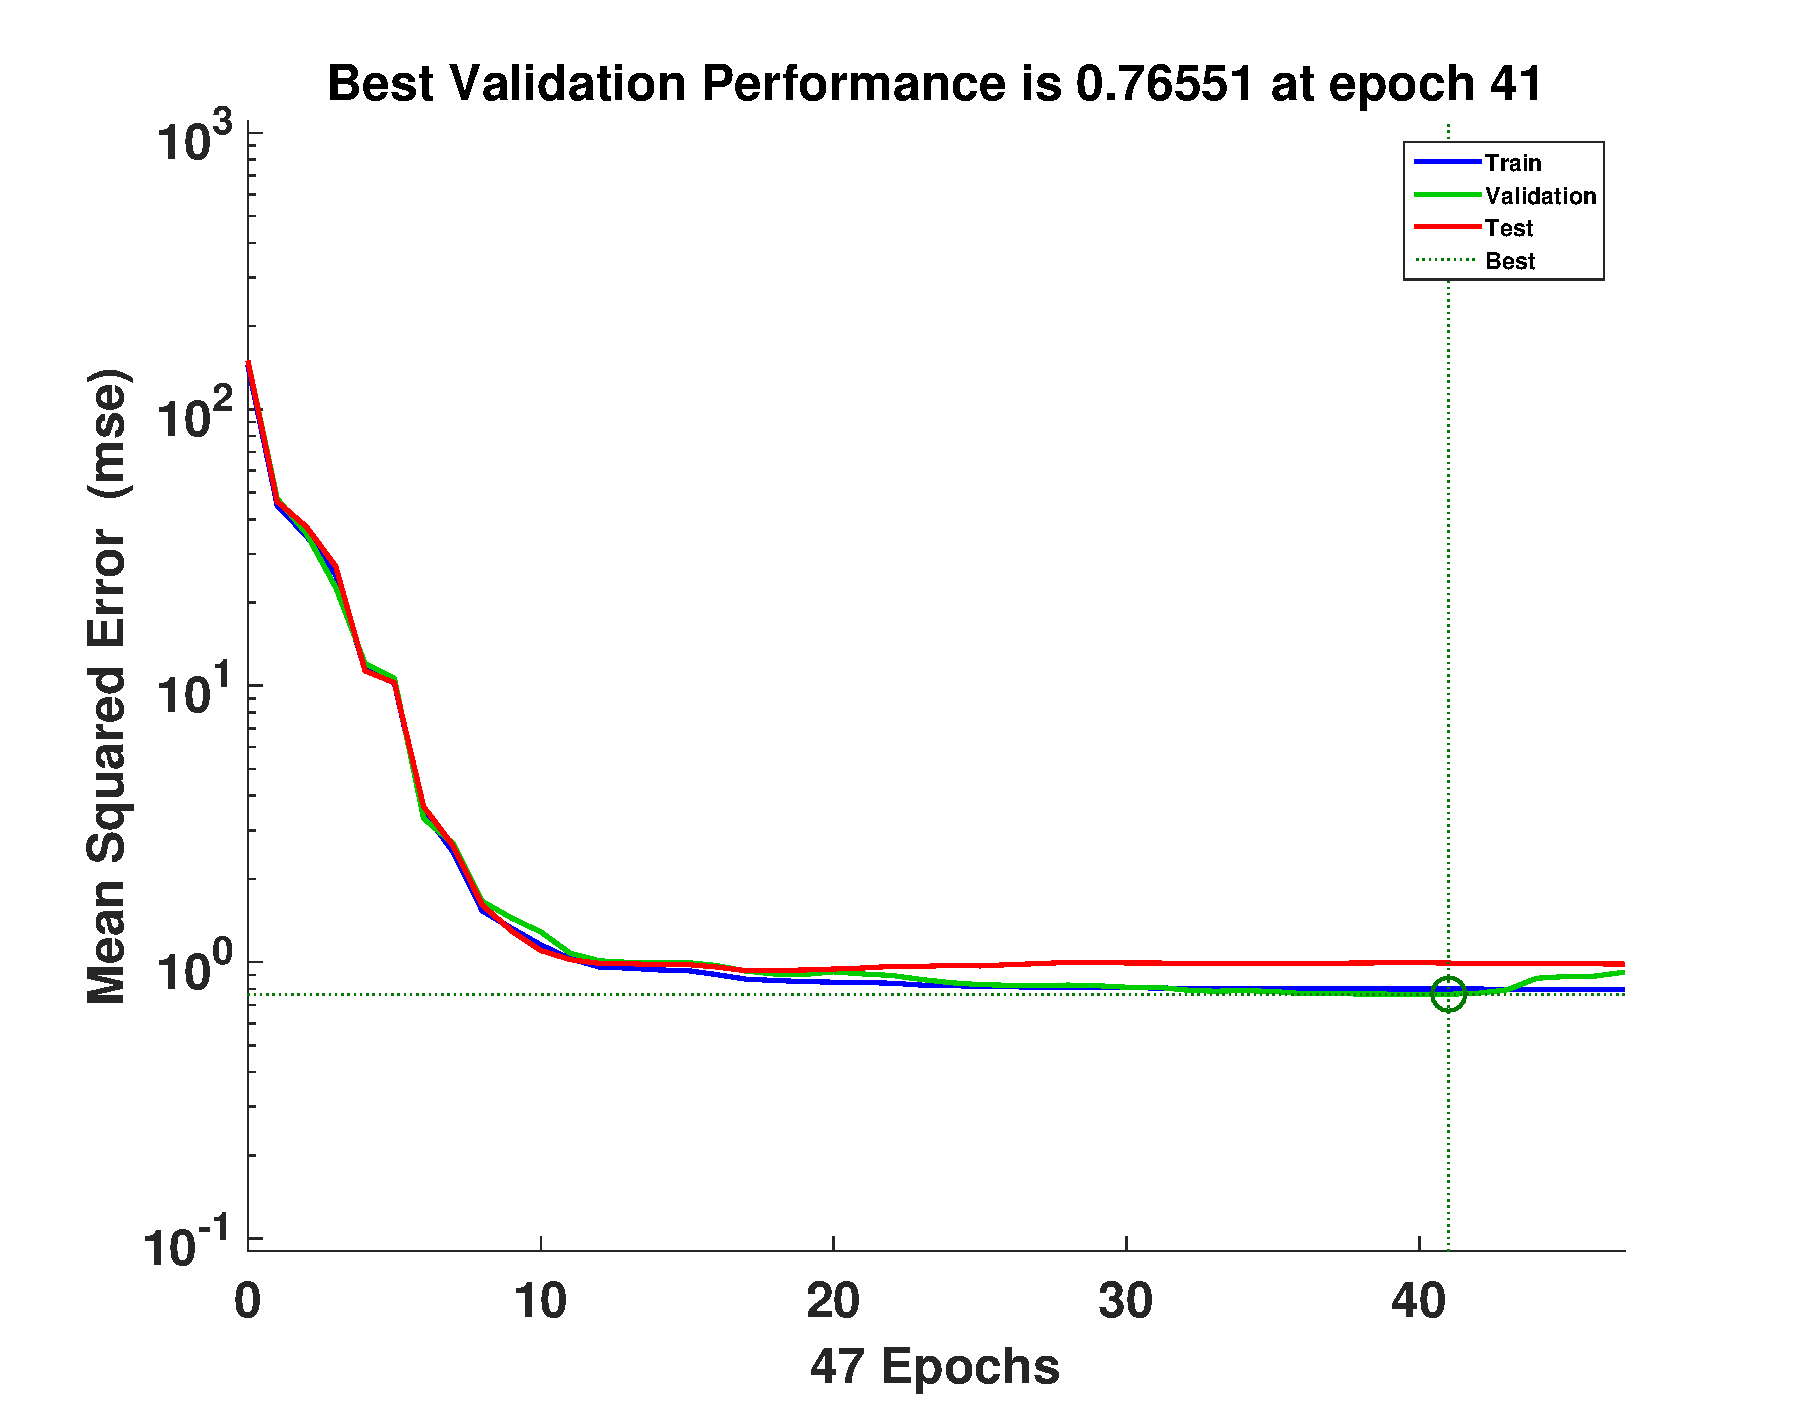
\includegraphics[width=4in]{./Pics/msr.eps}
\caption{Epoch and mean squared error.}
\label{fig:Epoch and mean squared error}
\end{figure}

Using a network large enough can provide an adequate fit to improve network generalization, because the functions of the whole network become more complex as the network gets larger. A small enough network is not able to fit the data well, however, neural network often faces over-fitting problem when it is applied into detection.

Fig. \ref{fig:Epoch and mean squared error} shows the curves of mean squared error for training data set, validation data set, and testing data set as epoch gets larger. At the beginning of the training, the mean squared error of three data set all rapidly drops, and the curves of the three different data set look quite close. After a certain time of epochs, the three curves begin to become flat, but the curve of validation data set still proceeds to decreases. At epoch 41, the validation performance achieves its best value 0.76651 which is the minimum of the whole curve of validation performance curve. After 6 epoches, the curve of the validation test still rises, therefore, 41 is selected as the best number for epoch in this model. As seen from the figure, the validation data set and test data set has quite close trends, which also indicates the overall data set are well divided.

\subsection{Analysis}
\begin{figure}[h]
\centering
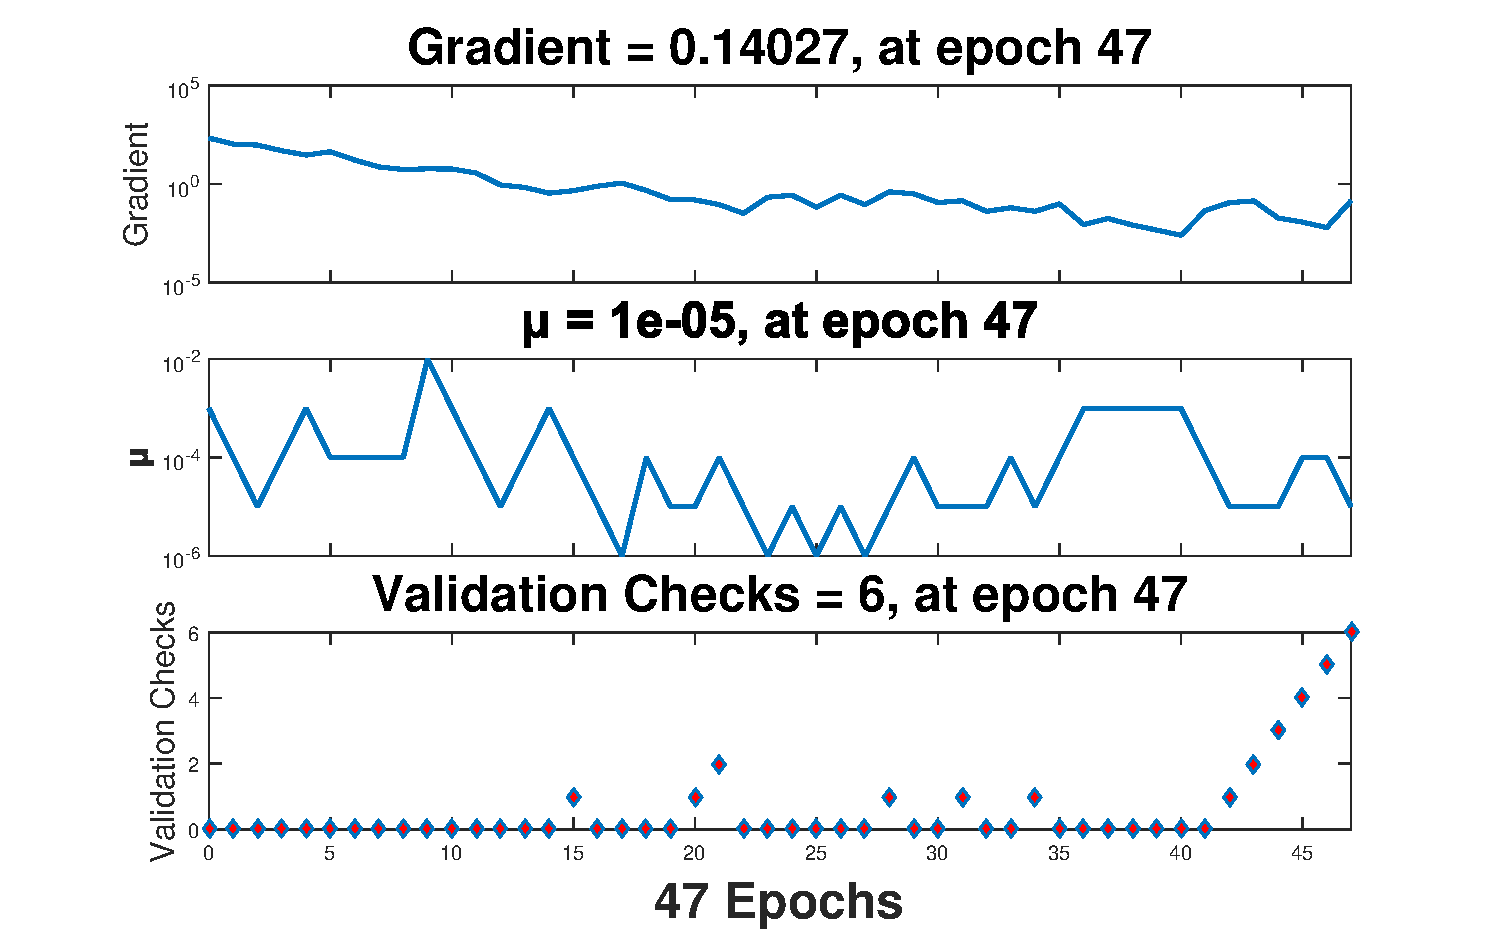
\includegraphics[width=4in]{./Pics/gradient.eps}
\caption{Gradient, $\mu$, and Validation Check.}
\label{fig:Gradient, Mu, and validation check.}
\end{figure}

\begin{figure}[h]
\centering
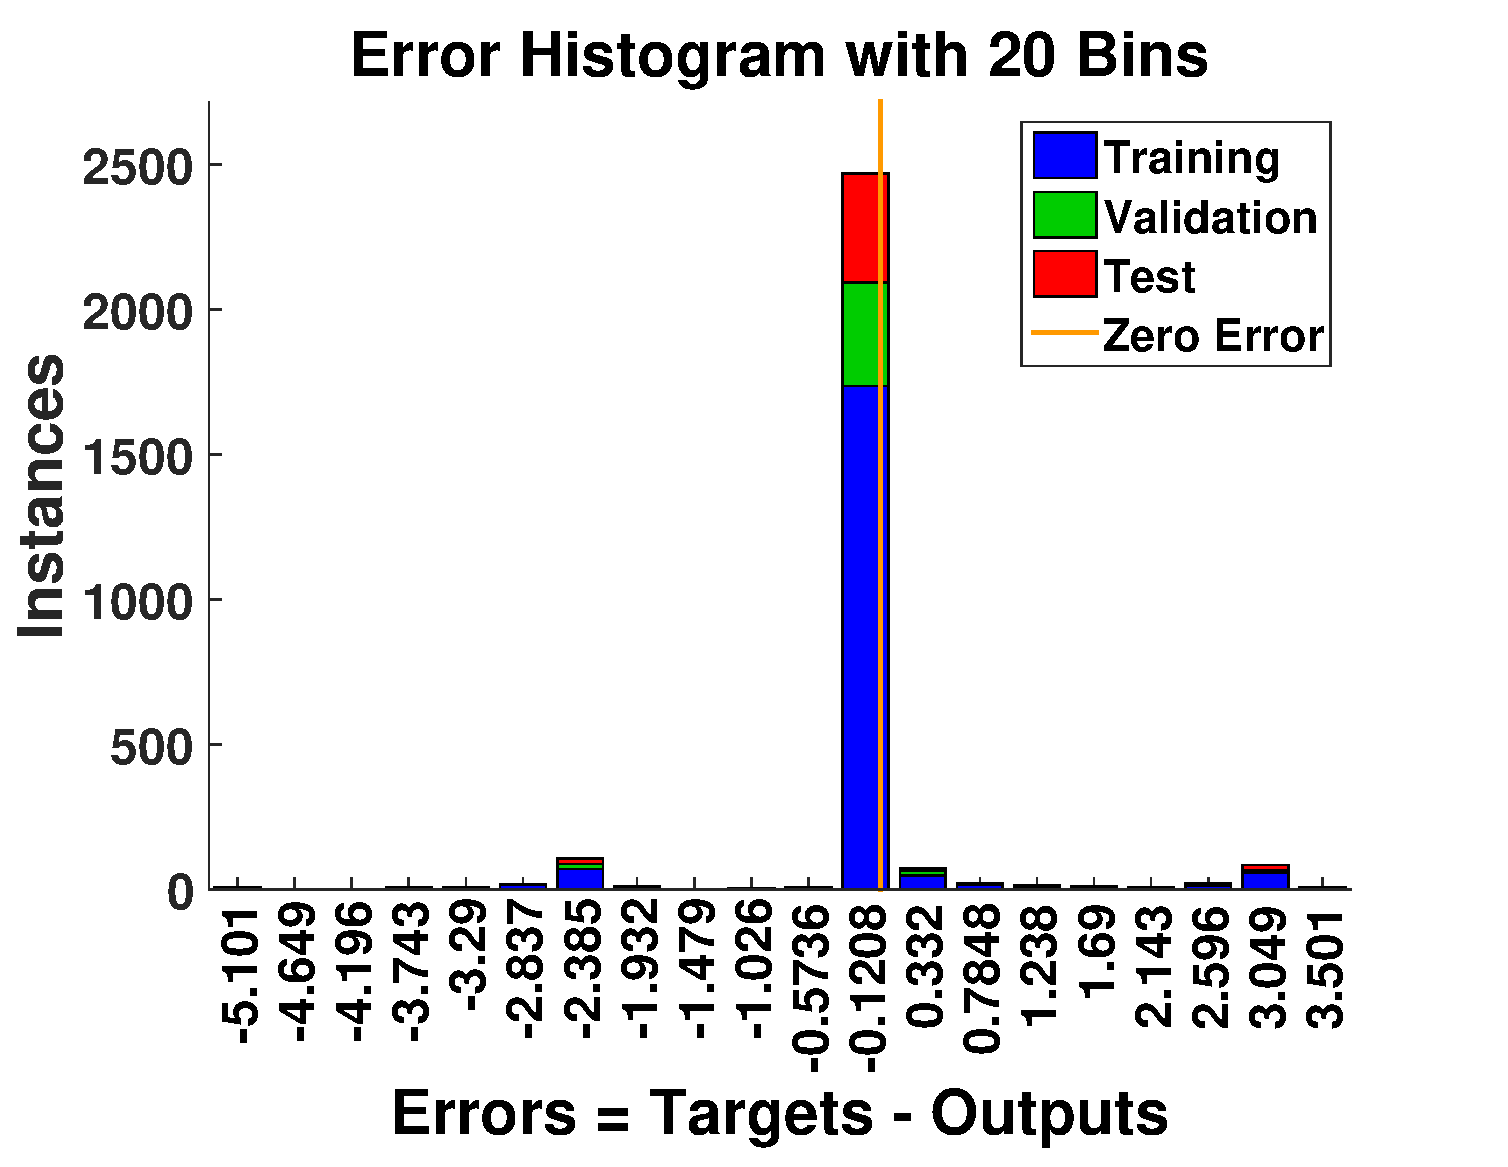
\includegraphics[width=4in]{./Pics/instances.eps}
\caption{Error histogram.}
\label{fig:Error histogram}
\end{figure}

One of the problems appearing to be very common in training neural network is over-fitting. Under this circumstance, the neural network conducts more iterations than necessary during the training process, which may lead to large error on testing data whereas the model performs well on the training data. The network has somehow memorized examples in training data, but fails in detecting data unknown.

To solve over-fitting problem existing in neural network, we apply for early stop method. As for all the data separation, we divide the whole data set into three divisions according to a certain proportion. With 70\% of data used for training, 15\% for validating, and 15\% for testing. Training data is presented to the neural network we build during training, which plays the role in adjusting weights and bias for network. Validation data is used to measure the degree to network generalization, which stops the training process if the performance of validation data starts to decline. Testing data has no impact on the whole training process which is an independent measure of network performance.

The number of iterations should be applied in training process depends on the curve change of validation error. During the initial phase of training, the validation error declines as the training set error declines. When the network starts to overfit the data, the error on validation set has a trend to go up. The training procedure is stopped under the situation that the validation error has increased for a certain number of iterations, and the network returns the weights and biases under current training when the validation error is at its minimum. In this model, 6 is a relatively safe number for the epoch to stop increasing, which means the training process is ceased when the validation test is monitored to have increased in row for 6 epoches. The test set error is applied for evaluating different models with different weights and biases, the plot of which is also giving a clear trend of how the test error changes. It implies a poor division of data if there is a significant variance between the test error and validating error.



\begin{figure}[h]
\centering
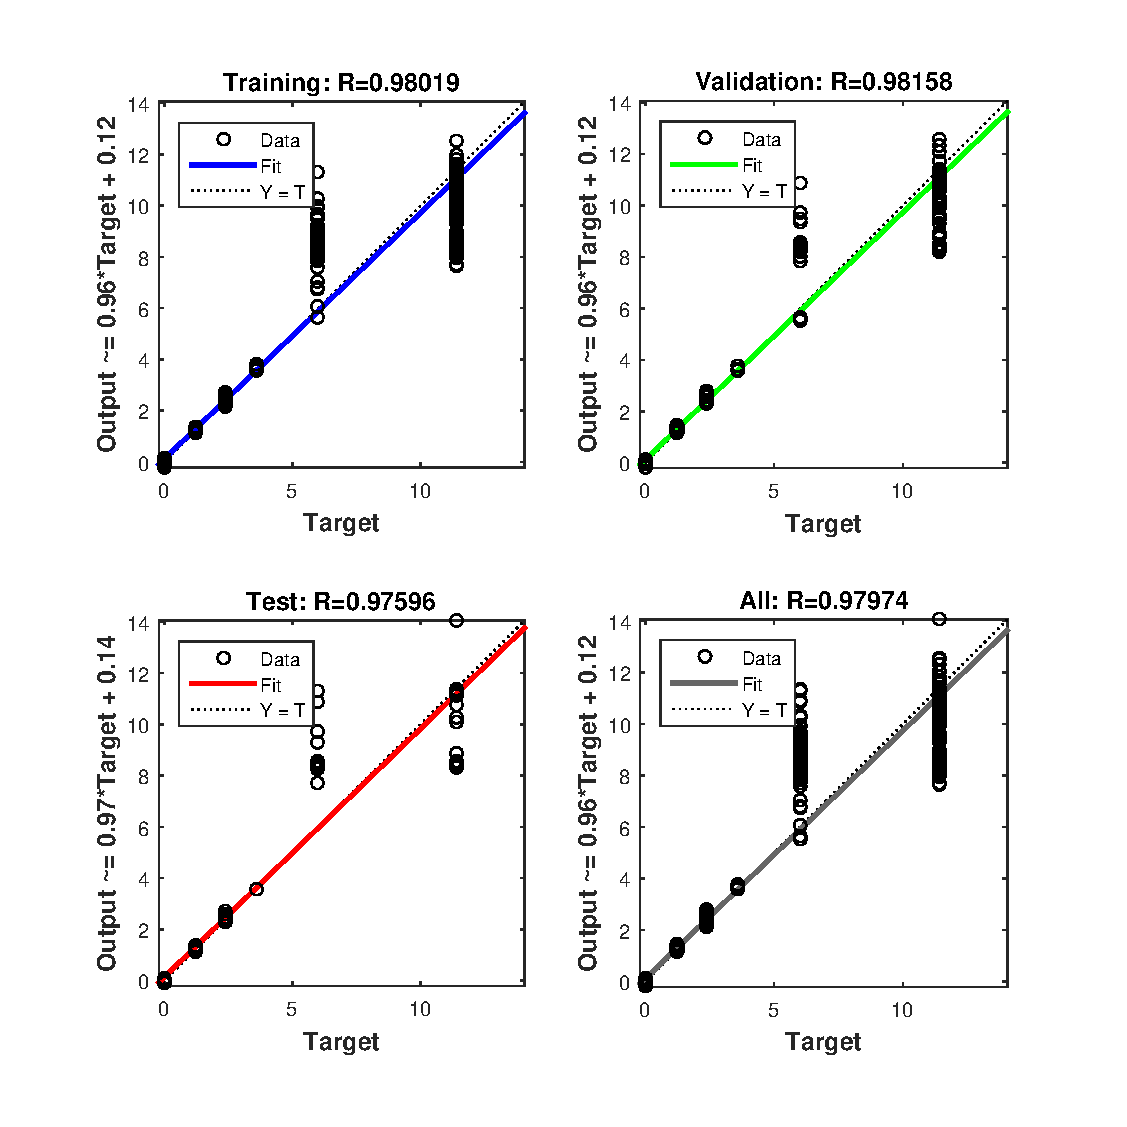
\includegraphics[width=5in]{./Pics/output.eps}
\caption{Regression check.}
\label{fig:Regression check}
\end{figure}

\begin{figure}[h]
\centering
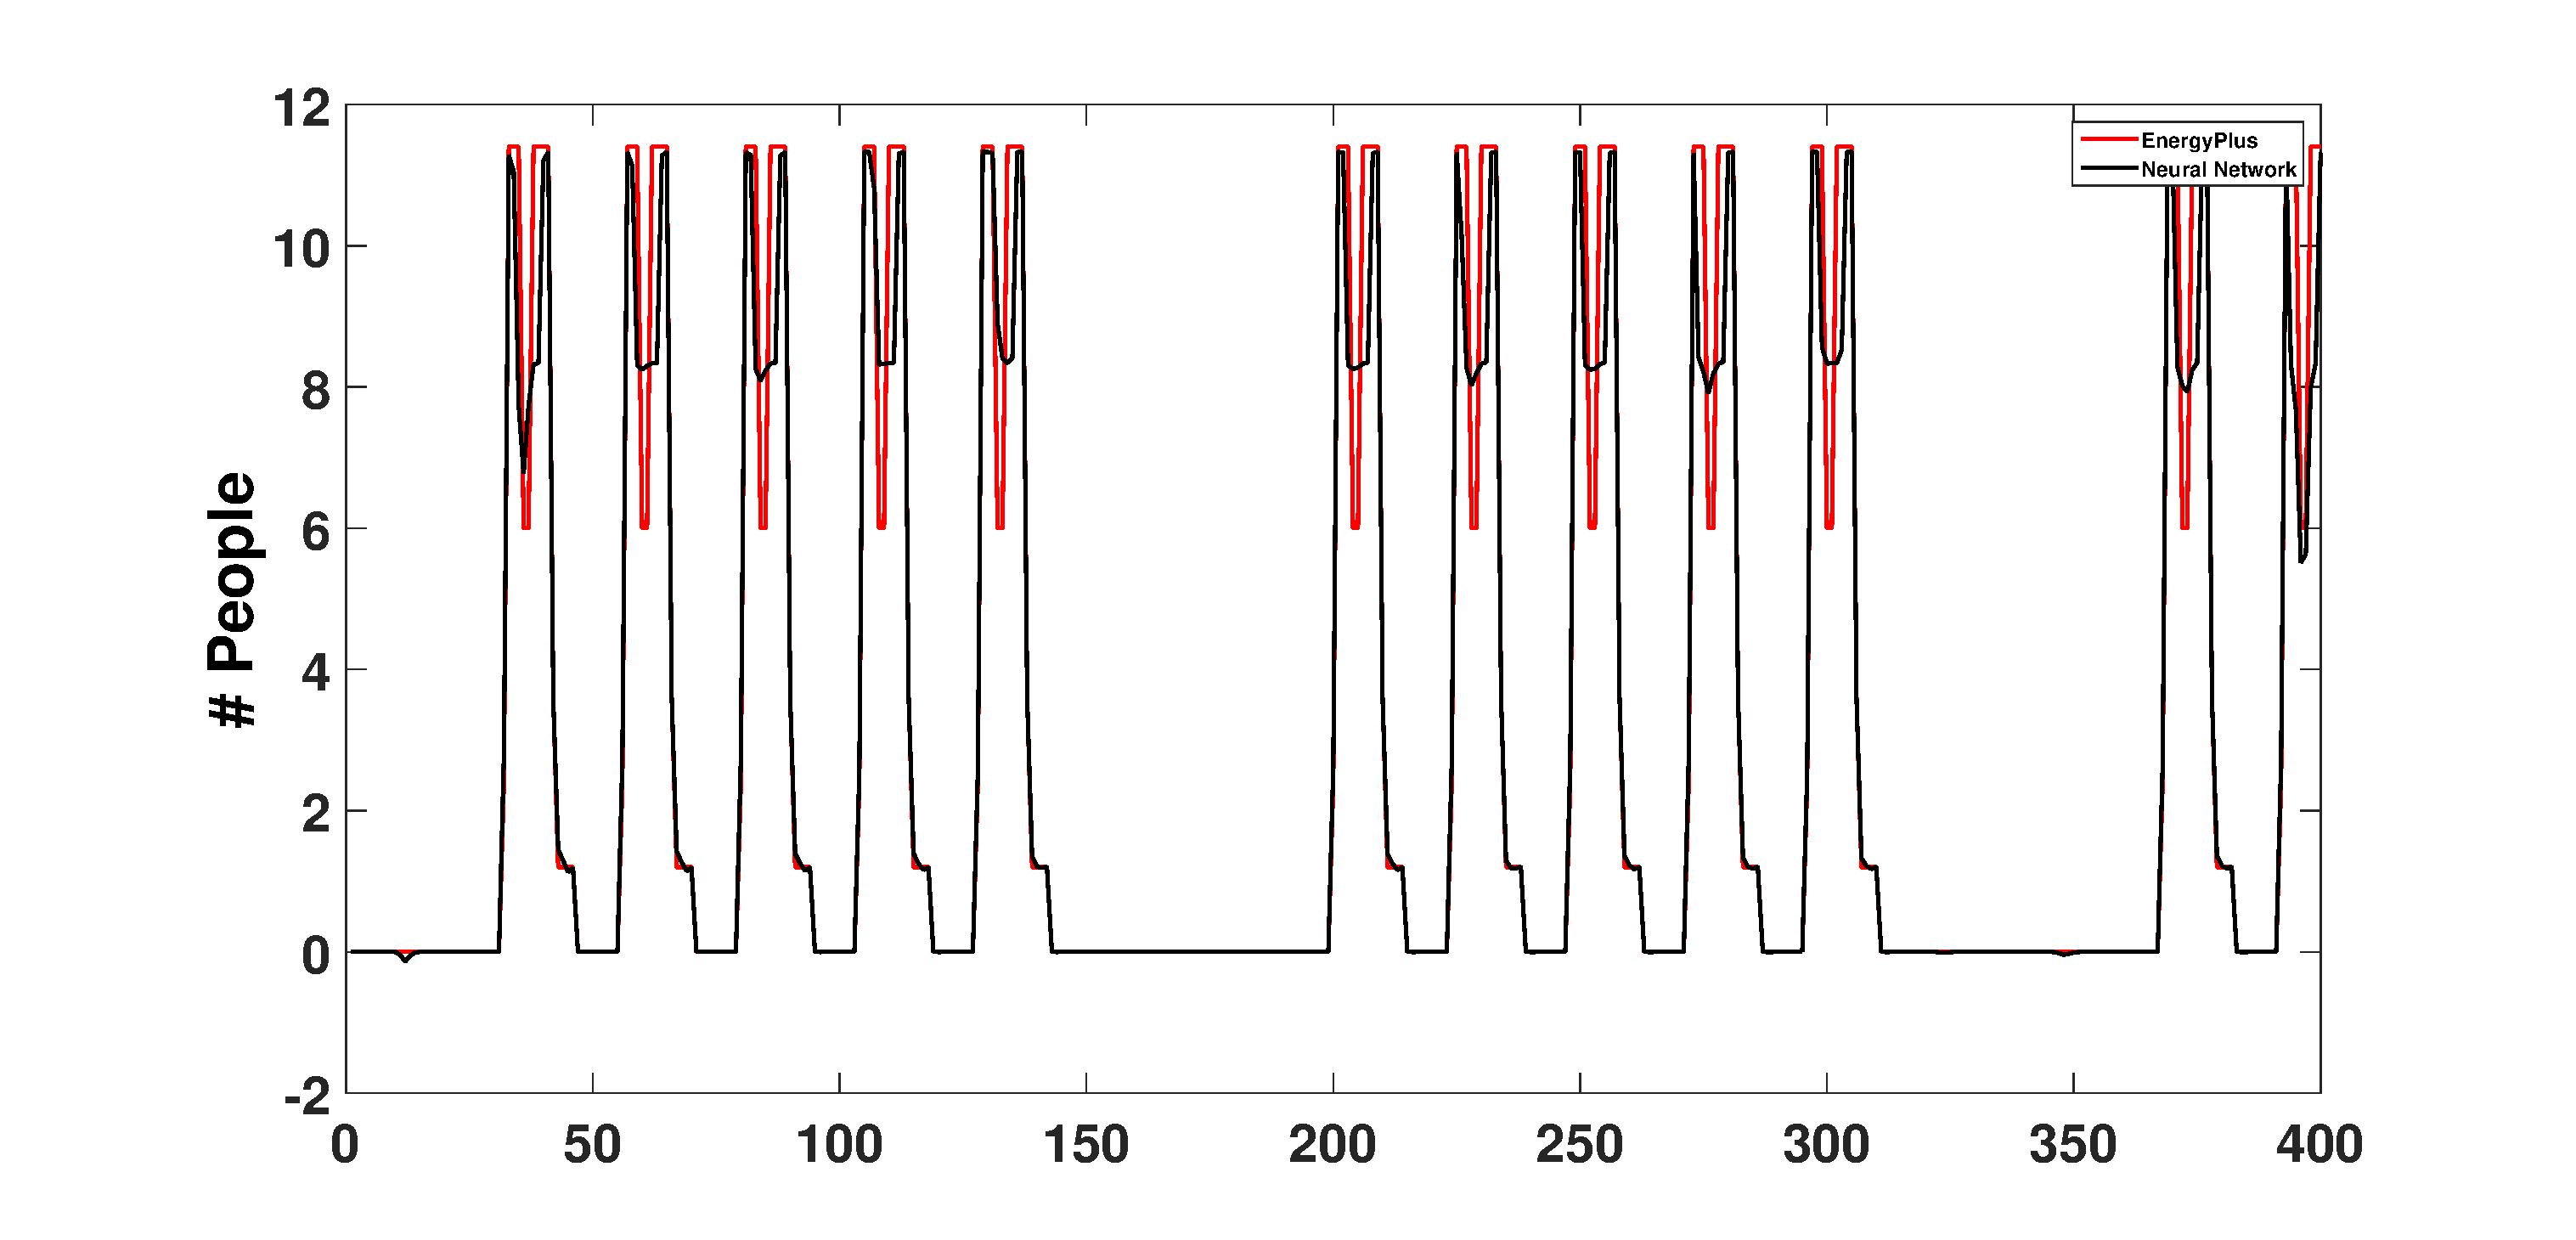
\includegraphics[width=5in]{./Pics/people.eps}
\caption{Occupancy estimation from neural network.}
\label{fig:occupancy estimation from neural network}
\end{figure}

Fig. \ref{fig:Gradient, Mu, and validation check.} shows curves of three different values in training procedure. The curve of gradient of the model constantly drops before epoch 41, and twisters for a few epoches before the epoch reaches 47. From the changing curve we can tell, 41 is a turning point for the training model, and it turns out to be the best ending epoch in this neural network. In comparison, the changing trend of $\mu$ curve is relatively not regular, but it turns out to get smaller on an overall perspective. At the bottom lies the validation check figure, as seen from the figure, the training process is ceased owing to the monitored straight 6 epoches increase in validation check, which well fits for the early stopping theory.

On Fig. \ref{fig:Error histogram}, the red bars denotes testing data, the green bars denotes validation data, and the blue bars denotes training data. Outliers can be easily spotted from the error histogram, for they fit apparently worse than most data points. If many data points are significantly different than the rest of the data points, it is suggested to check if there is some inherent in the original data set. More data points should be collected and trained in the neural network to detect the problem. As seen from Fig. \ref{fig:Error histogram}, the majority of errors lie close to the zero error mark, which signifies quite accurate fit for the neural network. Though there are some segments of error scatter a little distance from the zero error mark, the total number of them is comparatively low, which demonstrates that the neural network performs quite accurately in detecting outcome.

Regression is a statistical instrument for detecting the relationships among variables in statical modelling. The focus is on the relationship between different variables, and it includes many techniques and skills in modeling and analyzing variables. In essence, it is a helpful method to learn how a value of a variable changes when the other is varied or held fixed. More often than not, given the independent variables the regression analysis is able to estimate the conditioned expectation of the dependent variable. Fig. \ref{fig:Regression check} shows the regression analysis of the result produced through the neural network. The regression plots manifest the network outputs with respect to targets for training, validation, and test data sets. On a perfect regression, the data should match into a forty-five degression line where the targets equal the outputs from neural network. The four sub figures respectively represent the regression analysis for training, validation, test, and all. From the figures, the overall outputs have a relatively accurate value corresponding to targets. The value of R respectively for training, validation, test and all, is 0.98019, 0.98158, 0.97596 and 0.97974, which indicates that the neural network perform well in detecting unknown data points.

Fig. \ref{fig:occupancy estimation from neural network} shows the comparison of occupancy estimation between the original data points and the detected value from neural network. As seen from the figure, the overall accuracy of the detected value is relatively close, but there is a quite variation at the steepest part on the curve. We believe it is able to mitigate the variance by inducting more features to enhance the performance of neural network model.

From all above figures we can tell, the overall performance of neural network is relatively accurate. However, in contrast to mathematical based on SVR, the overall error is larger whereas the curve of the detected result fits better than its counterpart in SVR. In neural network, only 5-feature model is set up and it shows similar accuracy on occupancy detection. A conclusion is drawn from the comparison of the two different approaches that what influences the model more is the features and the number of data points while virtually the two different methods work similarly well for solving this problem.

\section{Conclusion}
In this paper, we propose a mathematical model respectively based on SVR and neural network to detect employee occupancy in a smart building. We use EnergyPlus, a realistic building thermal simulation software, to produce and collect training data and validation data with specific information about an office including building materials, walls, and roofs. In SVR model, two sets of features are offered to feed off the model for different conveniences. The first set of feature is comprised of 4 features including solar factor, working time, indoor temperature and outdoor temperature which are regarded as easily obtained features whereas the second set of features adds light energy as the fifth feature. In light of the experimental results, 4-feature model has a quite accurate detection rate which gives a 0.638 average error and 0.0532 error ratio. However, 5-feature SVR model giving a 0.317 average error and 0.0264 error ratio has a better performance than 4-feature model which we consider as moderating the under-fitting issue. This indicates using SVR model is a viable option when it comes to occupancy detection given its convenience in data acquirement. In neural network, only 5-feature model is established and it manifests similar accuracy on occupancy detection. A conclusion is drawn in this model that, what influences the model more is the features and the number of data points, virtually the two different methods work similarly well for solving this problem. However, further improvement is likely to occur when the model is refined to be able self-improved using current data set in the future.



% Bibliography
\bibliographystyle{ACM-Reference-Format-Journals}
\bibliography{title2}
                             % Sample .bib file with references that match those in
                             % the 'Specifications Document (V1.5)' as well containing
                             % 'legacy' bibs and bibs with 'alternate codings'.
                             % Gerry Murray - March 2012

% History dates
%\received{February 2007}{March 2009}{June 2009}

% Electronic Appendix
\elecappendix

\medskip



\end{document}
% End of v2-acmsmall-sample.tex (March 2012) - Gerry Murray, ACM


